\documentclass[12pt,a4paper]{article}
\usepackage[a4paper, margin=0.8in, headheight=14pt]{geometry}
\usepackage{fontspec}
\usepackage{unicode-math}
\setmainfont{TeX Gyre Pagella}
\setmonofont[Scale=0.88]{TeX Gyre Cursor}
\setmathfont{Latin Modern Math}
\usepackage{xcolor}
\usepackage{colortbl}
\usepackage{titlesec}
\usepackage{enumitem}
\usepackage{tabularx}
\usepackage{booktabs}
\usepackage{array}
\usepackage{amsmath}
\usepackage{tikz}
\usetikzlibrary{shapes.geometric, arrows.meta, positioning, calc, fit, decorations.pathreplacing, decorations.pathmorphing}
\usepackage{tcolorbox}
\tcbuselibrary{skins, breakable}
\usepackage{hyperref}
\usepackage{fancyhdr}
\usepackage{graphicx}
\usepackage{microtype}
\hyphenpenalty=10000
\exhyphenpenalty=10000
\sloppy
\usepackage{caption}
\usepackage{setspace}
\usepackage{multirow}
\usepackage{tocloft}
\newcommand{\Q}[1]{\textbf{#1}\par\noindent\ignorespaces}
\definecolor{myred}{RGB}{196,30,58}
\definecolor{mydark}{RGB}{30,30,50}
\definecolor{mygreen}{RGB}{14,120,80}
\definecolor{myteal}{RGB}{0,130,140}
\definecolor{myamber}{RGB}{180,100,0}
\definecolor{mypurple}{RGB}{100,30,160}
\definecolor{mygray}{RGB}{246,247,249}
\definecolor{mgframe}{RGB}{180,185,200}
\definecolor{watermark}{RGB}{145,150,170}
\definecolor{hdrred}{RGB}{250,232,235}
\definecolor{hdrgreen}{RGB}{220,244,233}
\definecolor{hdrteal}{RGB}{220,242,244}
\definecolor{hdramber}{RGB}{253,242,215}
\definecolor{hdrpurple}{RGB}{238,228,255}
\definecolor{hdrgray}{RGB}{238,240,245}
\definecolor{rowalt}{RGB}{250,251,253}

\titleformat{\section}{\large\bfseries\color{myred}}{\thesection.}{0.5em}{}[\vspace{1pt}{\color{myred}\rule{\linewidth}{0.8pt}}]
\titleformat{\subsection}{\normalsize\bfseries\color{myteal}}{\thesubsection}{0.5em}{}
\titlespacing*{\section}{0pt}{18pt}{7pt}
\titlespacing*{\subsection}{0pt}{11pt}{4pt}
\setlength{\parindent}{0pt}
\setlength{\parskip}{4pt}
\renewcommand{\cfttoctitlefont}{\large\bfseries\color{myred}}
\renewcommand{\cftaftertoctitle}{\par\noindent{\color{myred}\rule{\linewidth}{0.8pt}}}
\setlength{\cftbeforetoctitleskip}{0pt}
\setlength{\cftaftertoctitleskip}{6pt}
\renewcommand{\cftsecfont}{\normalsize\bfseries\color{mydark}}
\renewcommand{\cftsecpagefont}{\normalsize\bfseries\color{mydark}}
\renewcommand{\cftsecleader}{\cftdotfill{\cftdotsep}}
\setlength{\cftbeforesecskip}{7pt}
\renewcommand{\cftsubsecfont}{\small\color{mydark}}
\renewcommand{\cftsubsecpagefont}{\small\color{mydark}}
\setlength{\cftbeforesubsecskip}{3pt}
\setlength{\cftsubsecindent}{1.4em}
\renewcommand{\cftpartfont}{\normalsize\bfseries\color{myteal}}
\renewcommand{\cftpartpagefont}{\normalsize\bfseries\color{myteal}}
\setlength{\cftbeforepartskip}{14pt}
\renewcommand{\arraystretch}{1.45}
\setlength{\tabcolsep}{6pt}
\arrayrulecolor{mydark}
\newcolumntype{B}[1]{>{\small\bfseries\raggedright\arraybackslash}m{#1}}
\newcolumntype{C}[1]{>{\centering\arraybackslash}m{#1}}
\newcolumntype{Y}{>{\small\raggedright\arraybackslash}X}
\renewcommand{\tabularxcolumn}[1]{m{#1}}
\newcommand{\currmodule}{Module 1}
\pagestyle{fancy}
\fancyhf{}
\fancyhead[L]{\small\color{myred}\textbf{BS-CH101}\;\color{mydark}--- Chemistry-I}
\fancyhead[R]{\small\color{myteal}\textbf{\currmodule\ Notes}}
\fancyfoot[C]{\small\color{mydark}\thepage}
\fancyfoot[R]{\small\color{watermark}\textit{\copyright\ Biraj}}
\renewcommand{\headrulewidth}{0.5pt}
\renewcommand{\footrulewidth}{0.3pt}

\hypersetup{colorlinks=true, linkcolor=myteal, urlcolor=myteal,
  pdfauthor={Biraj Sarkar},
  pdftitle={BS-CH101 --- Combined Notes}}

\tcbset{
  tikzbox/.style={
    colback=mygray, colframe=mgframe, boxrule=0.6pt, arc=4pt,
    left=8pt, right=8pt, top=6pt, bottom=6pt,
    colbacktitle=mgframe, coltitle=mydark,
    fonttitle=\small\bfseries
  },
  defbox/.style={
    colback=hdrgreen, colframe=mygreen, boxrule=0.8pt, arc=4pt,
    left=9pt, right=9pt, top=6pt, bottom=6pt,
    colbacktitle=mygreen, coltitle=white,
    fonttitle=\small\bfseries
  },
  formulabox/.style={
    colback=hdrteal, colframe=myteal, boxrule=0.8pt, arc=4pt,
    left=9pt, right=9pt, top=7pt, bottom=7pt,
    colbacktitle=myteal, coltitle=white,
    fonttitle=\small\bfseries
  },
  examplebox/.style={
    colback=hdramber, colframe=myamber, boxrule=0.8pt, arc=4pt,
    left=9pt, right=9pt, top=6pt, bottom=6pt,
    colbacktitle=myamber, coltitle=white,
    fonttitle=\small\bfseries
  },
  masonbox/.style={
    colback=hdrpurple, colframe=mypurple, boxrule=0.8pt, arc=4pt,
    left=9pt, right=9pt, top=6pt, bottom=6pt,
    colbacktitle=mypurple, coltitle=white,
    fonttitle=\small\bfseries
  },
  exambox/.style={
    colback=hdrpurple, colframe=mypurple, boxrule=1pt, arc=5pt,
    left=10pt, right=10pt, top=8pt, bottom=8pt,
    colbacktitle=mypurple, coltitle=white,
    fonttitle=\bfseries,
    breakable, title after break={\textbf{Frequently Asked / Viva Questions (contd.)}}}
}
\tcbset{breakable}
\tcbset{after={\color{black}}}

\tikzset{
  block/.style={rectangle, draw=myteal, fill=hdrteal,
    text width=2.4cm, align=center, minimum height=0.95cm,
    font=\small, rounded corners=3pt, line width=0.7pt},
  redblock/.style={rectangle, draw=myred, fill=hdrred,
    text width=2.4cm, align=center, minimum height=0.95cm,
    font=\small, rounded corners=3pt, line width=0.7pt},
  netnode/.style={rectangle, draw=myteal, fill=hdrteal,
    text width=1.5cm, align=center, minimum height=0.8cm,
    font=\small, rounded corners=3pt, line width=0.7pt},
  sumjunc/.style={circle, draw=myamber, fill=hdramber,
    minimum size=0.62cm, font=\small, line width=0.8pt},
  snode/.style={circle, draw=mypurple, fill=hdrpurple,
    minimum size=0.55cm, font=\footnotesize, line width=0.7pt},
  arrow/.style={-Stealth, thick, color=mydark},
  redarrow/.style={-Stealth, thick, color=myred},
  line/.style={thick, color=mydark}
}

\newcommand{\modulestart}[2]{%
  \clearpage
  \renewcommand{\currmodule}{Module #1}%
  \renewcommand{\theHsection}{mod#1.\arabic{section}}%
  \renewcommand{\theHsubsection}{\theHsection.\arabic{subsection}}%
  \renewcommand{\theHsubsubsection}{\theHsubsection.\arabic{subsubsection}}%
  \phantomsection
  \addcontentsline{toc}{part}{Module #1: #2}%
  \setcounter{section}{0}%
  \begin{center}
    \vspace*{1.0cm}
    {\Huge\bfseries\color{myred} Module #1}\\[10pt]
    {\Large\bfseries\color{mydark} #2}\\[10pt]
    {\color{myred}\rule{0.55\linewidth}{1.2pt}}
  \end{center}
  \vspace{14pt}
}
\begin{document}

\thispagestyle{empty}
\vspace*{1.0cm}
\begin{center}
  {\Huge\bfseries\color{myred} BS-CH101}\\[10pt]
  {\LARGE\bfseries\color{mydark} Chemistry-I}\\[20pt]
  {\color{myred}\rule{0.7\linewidth}{1.5pt}}\\[18pt]
  {\Large\color{myteal}\textbf{Combined Module Notes}}\\[8pt]
  {\large\color{mydark} Modules 1 -- 7}\\[40pt]
  {\normalsize\color{mydark} Semester I \quad$\bullet$\quad 3L:1T:0P \quad$\bullet$\quad 4 Credits}\\[12pt]
  {\normalsize\color{mydark} CGEC \;$|$\; B.Tech ECE (2023--27)}\\[6pt]
  {\normalsize\color{mydark}\textit{Biraj Sarkar}}
\end{center}
\vspace{1.0cm}
\begin{center}
  \begin{tcolorbox}[colback=mygray, colframe=mgframe, boxrule=0.5pt, arc=3pt, width=0.85\linewidth]
    \centering\small\color{mydark}
    \textbf{Disclaimer / Study Guide Notice:}\\
    These are condensed \textbf{Short Notes} focusing on core theory, key formulas, block/circuit diagrams, and standard viva Q\&As for university exam revision. Exhaustive numerical practice problems and derivation edge cases are not covered. This serves as a quick-revision reference guide for students.
  \end{tcolorbox}
\end{center}
\vfill
\begin{center}{\small\color{watermark}\textit{Exam-Ready Notes}}\end{center}
\clearpage

\hypersetup{linkcolor=mydark}
\tableofcontents
\hypersetup{linkcolor=myteal}
\clearpage

% -- Module 1 -----------------------------------------------------------------
\modulestart{1}{Atomic and Molecular Structure}

\section{Atomic and Molecular Structure}
% ===============================================================================

\begin{tcolorbox}[defbox]
\textbf{Atomic and molecular structure} explains the arrangement of electrons in atoms and molecules, the origin of bonding, and the connection between energy levels and observable properties.
\end{tcolorbox}

\subsection{Schrodinger Wave Equation}
In quantum chemistry, an electron is described by a wave function $\psi$. The square of the wave function gives probability density, so $|\psi|^2 d\tau$ is the probability of finding the electron in a small volume element $d\tau$.

\begin{tcolorbox}[formulabox, title={Time-Independent Schrodinger Equation}]
\[
\hat{H}\psi = E\psi
\]
where $\hat{H}$ is the Hamiltonian operator, $\psi$ is the wave function, and $E$ is the permitted energy. For a one-dimensional particle,
\[
-\frac{h^2}{8\pi^2m}\frac{d^2\psi}{dx^2}+V\psi=E\psi
\]
\end{tcolorbox}

\subsection{Particle in a One-Dimensional Box}
For a particle confined between $x=0$ and $x=L$, the potential energy is zero inside the box and infinite outside it. Boundary conditions are:
\[
\psi(0)=0,\qquad \psi(L)=0
\]
The allowed wave functions and energies are:
\[
\psi_n=\sqrt{\frac{2}{L}}\sin\frac{n\pi x}{L},\qquad E_n=\frac{n^2h^2}{8mL^2},\quad n=1,2,3,\ldots
\]

\begin{tcolorbox}[tikzbox, title={Particle in a Box: Quantized Standing Waves}]
\centering
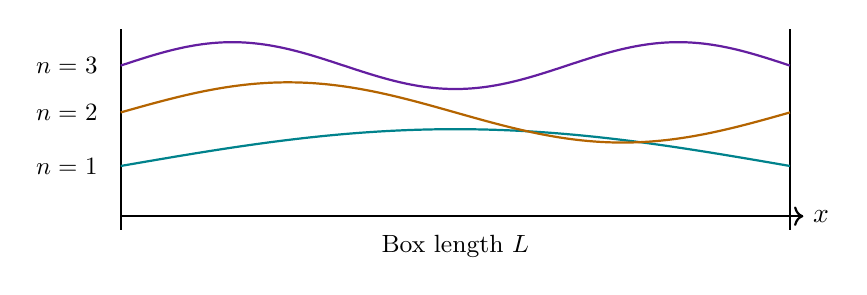
\begin{tikzpicture}[scale=0.85]
  \draw[->, thick] (0,0) -- (10.2,0) node[right] {$x$};
  \draw[thick] (0,-0.2) -- (0,2.8);
  \draw[thick] (10,-0.2) -- (10,2.8);
  \draw[myteal, thick, domain=0:10, samples=100] plot(\x,{0.75+0.55*sin(18*\x)});
  \draw[myamber, thick, domain=0:10, samples=120] plot(\x,{1.55+0.45*sin(36*\x)});
  \draw[mypurple, thick, domain=0:10, samples=140] plot(\x,{2.25+0.35*sin(54*\x)});
  \node[anchor=east, font=\small] at (-0.2,0.75) {$n=1$};
  \node[anchor=east, font=\small] at (-0.2,1.55) {$n=2$};
  \node[anchor=east, font=\small] at (-0.2,2.25) {$n=3$};
  \node[font=\small] at (5,-0.45) {Box length $L$};
\end{tikzpicture}
\end{tcolorbox}

\subsection{Molecular Orbitals of Diatomic Molecules}
Molecular orbital (MO) theory states that atomic orbitals combine to form molecular orbitals spread over the whole molecule. Constructive overlap gives bonding MOs and destructive overlap gives antibonding MOs.

\begin{tcolorbox}[formulabox, title={Bond Order}]
\[
\text{Bond order}=\frac{N_b-N_a}{2}
\]
where $N_b$ is the number of electrons in bonding MOs and $N_a$ is the number of electrons in antibonding MOs. Higher bond order means shorter, stronger bond.
\end{tcolorbox}

\textbf{Important examples:}\par\noindent
\begin{tabularx}{\linewidth}{|B{2.8cm}|Y|Y|Y|}
\hline
\textbf{Molecule} & \textbf{Configuration idea} & \textbf{Bond order} & \textbf{Magnetism} \\
\hline
$\mathrm{H_2}$ & Two electrons in $\sigma_{1s}$ & 1 & Diamagnetic \\
\hline
\hline
\end{tabularx}

\begin{tcolorbox}[tikzbox, title={Molecular Orbital Energy Level Diagram of Oxygen (\texorpdfstring{$\mathrm{O_2}$}{O2})}]
\centering
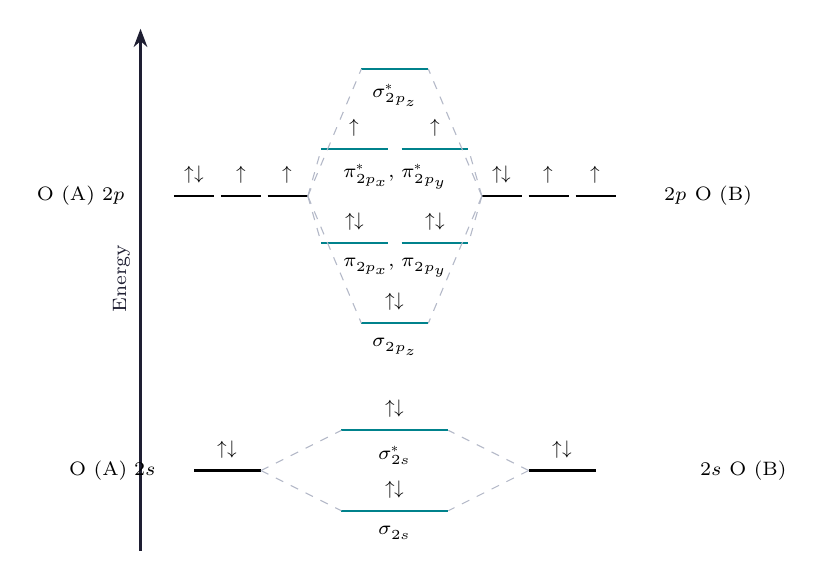
\begin{tikzpicture}[scale=0.85, every node/.style={font=\scriptsize}]
  % Energy axis on the left
  \draw[arrow] (-3.8,-2.6) -- (-3.8,5.2) node[midway, rotate=90, above=4pt] {Energy};

  % --- 2s Orbitals ---
  % AO Left
  \draw[thick] (-3.0,-1.4) -- (-2.0,-1.4) node[left=1.2cm] {O (A) $2s$};
  \node[above=1pt] at (-2.5,-1.4) {$\uparrow\downarrow$};

  % AO Right
  \draw[thick] (2.0,-1.4) -- (3.0,-1.4) node[right=1.2cm] {$2s$ O (B)};
  \node[above=1pt] at (2.5,-1.4) {$\uparrow\downarrow$};

  % MO Center
  \draw[thick, myteal] (-0.8,-2.0) -- (0.8,-2.0);
  \node[below=2pt] at (0,-2.0) {$\sigma_{2s}$};
  \node[above=1pt] at (0,-2.0) {$\uparrow\downarrow$};
  
  \draw[thick, myteal] (-0.8,-0.8) -- (0.8,-0.8);
  \node[below=2pt] at (0,-0.8) {$\sigma^*_{2s}$};
  \node[above=1pt] at (0,-0.8) {$\uparrow\downarrow$};

  % Connecting lines for 2s
  \draw[dashed, mgframe] (-2.0,-1.4) -- (-0.8,-2.0);
  \draw[dashed, mgframe] (-2.0,-1.4) -- (-0.8,-0.8);
  \draw[dashed, mgframe] (2.0,-1.4) -- (0.8,-2.0);
  \draw[dashed, mgframe] (2.0,-1.4) -- (0.8,-0.8);


  % --- 2p Orbitals ---
  % AO Left
  \draw[thick] (-3.3,2.7) -- (-2.7,2.7);
  \draw[thick] (-2.6,2.7) -- (-2.0,2.7);
  \draw[thick] (-1.9,2.7) -- (-1.3,2.7);
  \node[left=2.2cm] at (-1.3,2.7) {O (A) $2p$};
  \node[above=1pt] at (-3.0,2.7) {$\uparrow\downarrow$};
  \node[above=1pt] at (-2.3,2.7) {$\uparrow$};
  \node[above=1pt] at (-1.6,2.7) {$\uparrow$};

  % AO Right
  \draw[thick] (1.3,2.7) -- (1.9,2.7);
  \draw[thick] (2.0,2.7) -- (2.6,2.7);
  \draw[thick] (2.7,2.7) -- (3.3,2.7);
  \node[right=2.2cm] at (1.3,2.7) {$2p$ O (B)};
  \node[above=1pt] at (1.6,2.7) {$\uparrow\downarrow$};
  \node[above=1pt] at (2.3,2.7) {$\uparrow$};
  \node[above=1pt] at (3.0,2.7) {$\uparrow$};

  % MO Center
  \draw[thick, myteal] (-0.5,0.8) -- (0.5,0.8);
  \node[below=2pt] at (0,0.8) {$\sigma_{2p_z}$};
  \node[above=1pt] at (0,0.8) {$\uparrow\downarrow$};

  \draw[thick, myteal] (-1.1,2.0) -- (-0.1,2.0);
  \draw[thick, myteal] (0.1,2.0) -- (1.1,2.0);
  \node[below=2pt] at (0,2.0) {$\pi_{2p_x},\,\pi_{2p_y}$};
  \node[above=1pt] at (-0.6,2.0) {$\uparrow\downarrow$};
  \node[above=1pt] at (0.6,2.0) {$\uparrow\downarrow$};

  \draw[thick, myteal] (-1.1,3.4) -- (-0.1,3.4);
  \draw[thick, myteal] (0.1,3.4) -- (1.1,3.4);
  \node[below=2pt] at (0,3.4) {$\pi^*_{2p_x},\,\pi^*_{2p_y}$};
  \node[above=1pt] at (-0.6,3.4) {$\uparrow$};
  \node[above=1pt] at (0.6,3.4) {$\uparrow$};

  \draw[thick, myteal] (-0.5,4.6) -- (0.5,4.6);
  \node[below=2pt] at (0,4.6) {$\sigma^*_{2p_z}$};

  % Connecting lines for 2p
  \draw[dashed, mgframe] (-1.3,2.7) -- (-0.5,0.8);
  \draw[dashed, mgframe] (-1.3,2.7) -- (-1.1,2.0);
  \draw[dashed, mgframe] (-1.3,2.7) -- (-1.1,3.4);
  \draw[dashed, mgframe] (-1.3,2.7) -- (-0.5,4.6);

  \draw[dashed, mgframe] (1.3,2.7) -- (0.5,0.8);
  \draw[dashed, mgframe] (1.3,2.7) -- (1.1,2.0);
  \draw[dashed, mgframe] (1.3,2.7) -- (1.1,3.4);
  \draw[dashed, mgframe] (1.3,2.7) -- (0.5,4.6);
\end{tikzpicture}
\end{tcolorbox}

\subsection{Pi-Molecular Orbitals and Aromaticity}
Pi-electrons in conjugated systems are delocalized. Benzene has six pi-electrons distributed over six carbon atoms, making it unusually stable.

\begin{tcolorbox}[defbox]
\textbf{Aromatic compound:} A cyclic, planar, fully conjugated molecule having $(4n+2)$ pi-electrons, where $n=0,1,2,\ldots$.
\end{tcolorbox}

\begin{tcolorbox}[tikzbox, title={Benzene Pi-Electron Delocalization}]
\centering
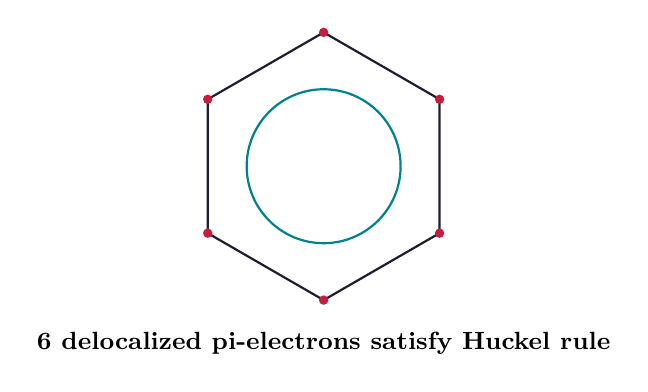
\begin{tikzpicture}[scale=0.85]
  \foreach \i in {1,...,6} {
    \coordinate (C\i) at ({90+60*(\i-1)}:2);
  }
  \draw[thick, color=mydark] (C1)--(C2)--(C3)--(C4)--(C5)--(C6)--cycle;
  \draw[myteal, thick] (0,0) circle (1.15);
  \foreach \i in {1,...,6} \fill[myred] (C\i) circle (2pt);
  \node[font=\small\bfseries] at (0,-2.65) {6 delocalized pi-electrons satisfy Huckel rule};
\end{tikzpicture}
\end{tcolorbox}

\subsection{Pi-Molecular Orbitals of 1,3-Butadiene}
1,3-butadiene ($\mathrm{CH_2=CH-CH=CH_2}$) has a conjugated system of four $p$ orbitals containing four $\pi$ electrons. These combine to form four $\pi$ molecular orbitals ($\psi_1, \psi_2, \psi_3, \psi_4$) with increasing energy and nodes.
\begin{itemize}[leftmargin=*, itemsep=3pt]
  \item \textbf{Nodal Properties:} The number of nodes in orbital $\psi_k$ is equal to $(k-1)$. A node is a position where the wave function changes sign and electron probability is zero.
  \item \textbf{HOMO/LUMO:} In the ground state, the four $\pi$ electrons fill the two lowest-energy orbitals ($\psi_1, \psi_2$). Thus, $\psi_2$ is the \textbf{Highest Occupied Molecular Orbital (HOMO)} and $\psi_3$ is the \textbf{Lowest Unoccupied Molecular Orbital (LUMO)}.
\end{itemize}

\begin{tcolorbox}[tikzbox, title={Pi-Molecular Orbitals of 1,3-Butadiene}]
\centering
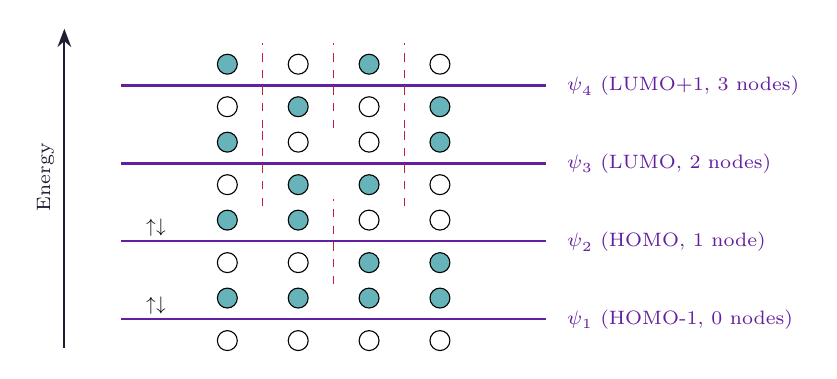
\begin{tikzpicture}[scale=0.9, every node/.style={font=\scriptsize}]
  % Energy axis
  \draw[arrow] (-3.8,-0.5) -- (-3.8,4.0) node[midway, rotate=90, above=4pt] {Energy};

  % --- Level psi_4 (3 nodes) ---
  \draw[thick, mypurple] (-3.0,3.2) -- (3.0,3.2) node[right=4pt] {$\psi_4$ (LUMO+1, 3 nodes)};
  % Draw lobes for + - + -
  \fill[myteal!60] (-1.5,3.5) circle (4pt); \draw (-1.5,3.5) circle (4pt);
  \draw (-1.5,2.9) circle (4pt);
  \draw (-0.5,3.5) circle (4pt);
  \fill[myteal!60] (-0.5,2.9) circle (4pt); \draw (-0.5,2.9) circle (4pt);
  \fill[myteal!60] (0.5,3.5) circle (4pt); \draw (0.5,3.5) circle (4pt);
  \draw (0.5,2.9) circle (4pt);
  \draw (1.5,3.5) circle (4pt);
  \fill[myteal!60] (1.5,2.9) circle (4pt); \draw (1.5,2.9) circle (4pt);
  % Nodes
  \draw[dashed, myred] (-1.0,2.6) -- (-1.0,3.8);
  \draw[dashed, myred] (0.0,2.6) -- (0.0,3.8);
  \draw[dashed, myred] (1.0,2.6) -- (1.0,3.8);

  % --- Level psi_3 (2 nodes) ---
  \draw[thick, mypurple] (-3.0,2.1) -- (3.0,2.1) node[right=4pt] {$\psi_3$ (LUMO, 2 nodes)};
  % Draw lobes for + - - +
  \fill[myteal!60] (-1.5,2.4) circle (4pt); \draw (-1.5,2.4) circle (4pt);
  \draw (-1.5,1.8) circle (4pt);
  \draw (-0.5,2.4) circle (4pt);
  \fill[myteal!60] (-0.5,1.8) circle (4pt); \draw (-0.5,1.8) circle (4pt);
  \draw (0.5,2.4) circle (4pt);
  \fill[myteal!60] (0.5,1.8) circle (4pt); \draw (0.5,1.8) circle (4pt);
  \fill[myteal!60] (1.5,2.4) circle (4pt); \draw (1.5,2.4) circle (4pt);
  \draw (1.5,1.8) circle (4pt);
  % Nodes
  \draw[dashed, myred] (-1.0,1.5) -- (-1.0,2.7);
  \draw[dashed, myred] (1.0,1.5) -- (1.0,2.7);

  % --- Level psi_2 (1 node) ---
  \draw[thick, mypurple] (-3.0,1.0) -- (3.0,1.0) node[right=4pt] {$\psi_2$ (HOMO, 1 node)};
  \node at (-2.5, 1.2) {$\uparrow\downarrow$};
  % Draw lobes for + + - -
  \fill[myteal!60] (-1.5,1.3) circle (4pt); \draw (-1.5,1.3) circle (4pt);
  \draw (-1.5,0.7) circle (4pt);
  \fill[myteal!60] (-0.5,1.3) circle (4pt); \draw (-0.5,1.3) circle (4pt);
  \draw (-0.5,0.7) circle (4pt);
  \draw (0.5,1.3) circle (4pt);
  \fill[myteal!60] (0.5,0.7) circle (4pt); \draw (0.5,0.7) circle (4pt);
  \draw (1.5,1.3) circle (4pt);
  \fill[myteal!60] (1.5,0.7) circle (4pt); \draw (1.5,0.7) circle (4pt);
  % Nodes
  \draw[dashed, myred] (0.0,0.4) -- (0.0,1.6);

  % --- Level psi_1 (0 nodes) ---
  \draw[thick, mypurple] (-3.0,-0.1) -- (3.0,-0.1) node[right=4pt] {$\psi_1$ (HOMO-1, 0 nodes)};
  \node at (-2.5, 0.1) {$\uparrow\downarrow$};
  % Draw lobes for + + + +
  \fill[myteal!60] (-1.5,0.2) circle (4pt); \draw (-1.5,0.2) circle (4pt);
  \draw (-1.5,-0.4) circle (4pt);
  \fill[myteal!60] (-0.5,0.2) circle (4pt); \draw (-0.5,0.2) circle (4pt);
  \draw (-0.5,-0.4) circle (4pt);
  \fill[myteal!60] (0.5,0.2) circle (4pt); \draw (0.5,0.2) circle (4pt);
  \draw (0.5,-0.4) circle (4pt);
  \fill[myteal!60] (1.5,0.2) circle (4pt); \draw (1.5,0.2) circle (4pt);
  \draw (1.5,-0.4) circle (4pt);
\end{tikzpicture}
\end{tcolorbox}

\subsection{Crystal Field Theory}
In transition-metal complexes, surrounding ligands split the five degenerate $d$ orbitals into different energy groups. The splitting controls colour, magnetic behaviour, and stability.

\begin{tcolorbox}[tikzbox, title={Octahedral Crystal Field Splitting}]
\centering
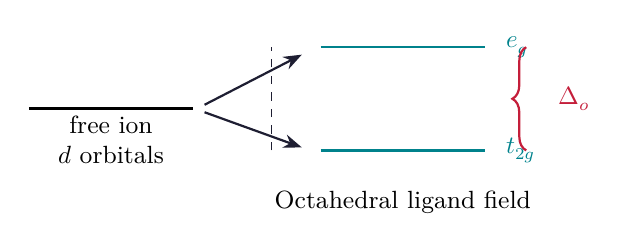
\begin{tikzpicture}[scale=0.95]
  \draw[thick] (0,0) -- (2.2,0);
  \node[font=\small, align=center] at (1.1,-0.42) {free ion\\$d$ orbitals};

  \draw[arrow] (2.35,0.05) -- (3.65,0.72);
  \draw[arrow] (2.35,-0.05) -- (3.65,-0.52);

  \draw[thick,myteal] (3.9,0.82) -- (6.1,0.82);
  \node[font=\small\bfseries\color{myteal}, anchor=west] at (6.25,0.82) {$e_g$};

  \draw[thick,myteal] (3.9,-0.56) -- (6.1,-0.56);
  \node[font=\small\bfseries\color{myteal}, anchor=west] at (6.25,-0.56) {$t_{2g}$};

  \draw[dashed,mydark] (3.25,-0.56) -- (3.25,0.82);
  \draw[decorate, decoration={brace, amplitude=5pt}, thick, myred] (6.65,-0.56) -- (6.65,0.82)
    node[midway,right=8pt,font=\small\bfseries\color{myred}] {$\Delta_o$};
  \node[font=\small] at (5.0,-1.25) {Octahedral ligand field};
\end{tikzpicture}
\end{tcolorbox}

\subsection{Band Structure and Doping}
In solids, many atomic orbitals combine to form bands. Conductivity depends on the band gap $E_g$ between valence band and conduction band.

\begin{tabularx}{\linewidth}{|B{3cm}|Y|Y|}
\hline
\textbf{Material} & \textbf{Band gap} & \textbf{Electrical behaviour} \\
\hline
Conductor & Overlapping bands or very small gap & Electrons move easily \\
\hline
Semiconductor & Moderate gap, about $1$--$3\ \mathrm{eV}$ & Conductivity increases by heat or doping \\
\hline
Insulator & Large gap, usually $>5\ \mathrm{eV}$ & Very poor conductor \\
\hline
\end{tabularx}

\begin{tcolorbox}[exambox, title={Exam Points}]
\begin{itemize}[leftmargin=*, itemsep=2pt, topsep=2pt]
  \item Derive $E_n=n^2h^2/(8mL^2)$ using boundary conditions.
  \item For MO questions, always calculate bond order and then state magnetic nature.
  \item For CFT, mention splitting pattern, $\Delta_o$, high spin or low spin, and magnetic moment.
  \item For band theory, draw valence band, conduction band, and band gap.
\end{itemize}
\end{tcolorbox}

% ===============================================================================
\section{Exam-Oriented Derivations and Applications}
% ===============================================================================

\subsection{Derivation of Particle in a Box Energy}
For a one-dimensional box, potential energy inside the box is zero. Therefore the Schrodinger equation becomes:
\[
-\frac{h^2}{8\pi^2m}\frac{d^2\psi}{dx^2}=E\psi
\]
Rearranging,
\[
\frac{d^2\psi}{dx^2}+\frac{8\pi^2mE}{h^2}\psi=0
\]
Let
\[
k^2=\frac{8\pi^2mE}{h^2}
\]
Then the differential equation becomes:
\[
\frac{d^2\psi}{dx^2}+k^2\psi=0
\]
Its general solution is:
\[
\psi=A\sin kx+B\cos kx
\]
Boundary condition at $x=0$ gives $B=0$. Boundary condition at $x=L$ gives:
\[
A\sin kL=0
\]
For a non-zero wave function:
\[
kL=n\pi,\qquad k=\frac{n\pi}{L}
\]
Substituting in $k^2=8\pi^2mE/h^2$:
\[
E_n=\frac{n^2h^2}{8mL^2}
\]

\begin{tcolorbox}[examplebox, title={Solved Example: Energy Level Ratio}]
\textbf{Problem:} Find the ratio of the first three energy levels for a particle in a box.

\textbf{Solution:} Since $E_n\propto n^2$,
\[
E_1:E_2:E_3=1^2:2^2:3^2=1:4:9
\]
\textbf{Exam note:} Energy gaps are not equal; they increase with $n$.
\end{tcolorbox}

\subsection{MO Filling Order and Magnetic Behaviour}
For second-period diatomic molecules, MO ordering changes after $\mathrm{N_2}$ because $s$-$p$ mixing becomes less important. This is a common exam trap.

\begin{tabularx}{\linewidth}{|B{3.5cm}|Y|Y|}
\hline
\textbf{Molecules} & \textbf{MO order to remember} & \textbf{Important result} \\
\hline
$\mathrm{B_2,C_2,N_2}$ & $\sigma_{2s}<\sigma^*_{2s}<\pi_{2p}<\sigma_{2p}<\pi^*_{2p}<\sigma^*_{2p}$ & $\mathrm{B_2}$ is paramagnetic; $\mathrm{N_2}$ has bond order 3 \\
\hline
$\mathrm{O_2,F_2,Ne_2}$ & $\sigma_{2s}<\sigma^*_{2s}<\sigma_{2p}<\pi_{2p}<\pi^*_{2p}<\sigma^*_{2p}$ & $\mathrm{O_2}$ is paramagnetic due to two unpaired electrons \\
\hline
\end{tabularx}

\begin{tcolorbox}[examplebox, title={Solved Example: Bond Order of Oxygen}]
For $\mathrm{O_2}$, total valence electrons are $12$.
\[
N_b=8,\qquad N_a=4
\]
\[
\text{Bond order}=\frac{8-4}{2}=2
\]
Two electrons remain unpaired in $\pi^*_{2p}$ orbitals, so oxygen is \textbf{paramagnetic}.
\end{tcolorbox}

\subsection{Crystal Field Splitting: High Spin and Low Spin}
In octahedral complexes, electrons first occupy lower $t_{2g}$ orbitals. Whether pairing occurs depends on the relative values of crystal field splitting energy $\Delta_o$ and pairing energy $P$.

\begin{tabularx}{\linewidth}{|B{3.2cm}|Y|Y|}
\hline
\textbf{Case} & \textbf{Condition} & \textbf{Result} \\
\hline
High spin complex & $\Delta_o<P$ & Electrons avoid pairing; more unpaired electrons; usually weak-field ligands \\
\hline
Low spin complex & $\Delta_o>P$ & Electrons pair in $t_{2g}$ before occupying $e_g$; fewer unpaired electrons; usually strong-field ligands \\
\hline
\end{tabularx}

\begin{tcolorbox}[tikzbox, title={High Spin and Low Spin Choice for Octahedral Complexes}]
\centering
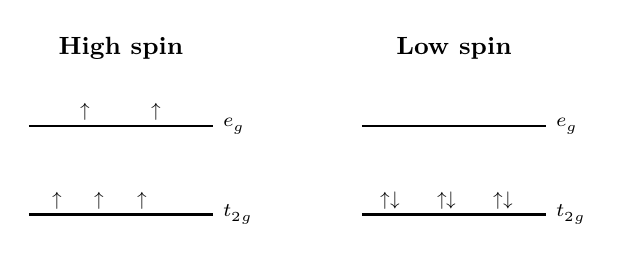
\begin{tikzpicture}[scale=0.9]
  \node[font=\small\bfseries] at (1.3,2.35) {High spin};
  \draw[thick] (0,0) -- (2.6,0) node[right,font=\scriptsize] {$t_{2g}$};
  \draw[thick] (0,1.25) -- (2.6,1.25) node[right,font=\scriptsize] {$e_g$};
  \foreach \x in {0.4,1.0,1.6} \node[font=\scriptsize] at (\x,0.2) {$\uparrow$};
  \foreach \x in {0.8,1.8} \node[font=\scriptsize] at (\x,1.45) {$\uparrow$};

  \node[font=\small\bfseries] at (6.0,2.35) {Low spin};
  \draw[thick] (4.7,0) -- (7.3,0) node[right,font=\scriptsize] {$t_{2g}$};
  \draw[thick] (4.7,1.25) -- (7.3,1.25) node[right,font=\scriptsize] {$e_g$};
  \foreach \x in {5.1,5.9,6.7} \node[font=\scriptsize] at (\x,0.2) {$\uparrow\downarrow$};
\end{tikzpicture}
\end{tcolorbox}

\subsection{n-Type and p-Type Semiconductors}
Doping adds controlled impurities to a semiconductor. Pentavalent dopants such as P or As introduce donor levels and produce n-type semiconductors. Trivalent dopants such as B or Al introduce acceptor levels and produce p-type semiconductors.

\begin{tcolorbox}[tikzbox, title={Doping Levels in Semiconductors}]
\centering
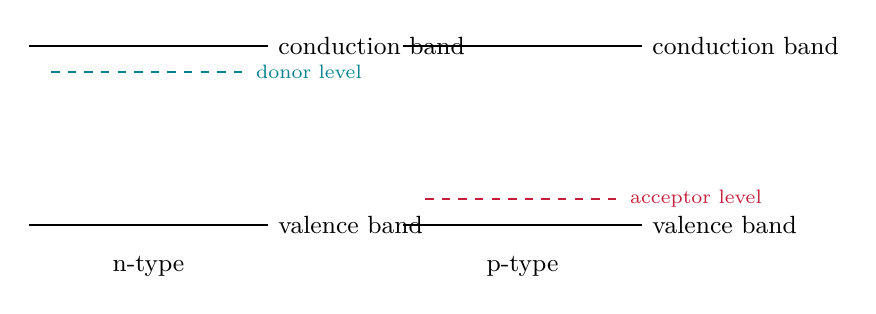
\begin{tikzpicture}[scale=0.95]
  \draw[thick] (0,0) -- (3.2,0) node[right,font=\small] {valence band};
  \draw[thick] (0,2.4) -- (3.2,2.4) node[right,font=\small] {conduction band};
  \draw[myteal, thick, dashed] (0.3,2.05) -- (2.9,2.05) node[right,font=\scriptsize] {donor level};
  \node[font=\small] at (1.6,-0.55) {n-type};

  \draw[thick] (5,0) -- (8.2,0) node[right,font=\small] {valence band};
  \draw[thick] (5,2.4) -- (8.2,2.4) node[right,font=\small] {conduction band};
  \draw[myred, thick, dashed] (5.3,0.35) -- (7.9,0.35) node[right,font=\scriptsize] {acceptor level};
  \node[font=\small] at (6.6,-0.55) {p-type};
\end{tikzpicture}
\end{tcolorbox}

\begin{tcolorbox}[masonbox, title={How to Write 10-Mark Answers in This Module}]
\begin{enumerate}[leftmargin=*, itemsep=3pt, topsep=2pt]
  \item Start with a definition in 2--3 lines.
  \item Draw the required energy-level or orbital diagram.
  \item Write the governing formula with symbol meanings.
  \item Add one example such as $\mathrm{O_2}$ paramagnetism, benzene aromaticity, or n-type doping.
  \item End with one application or exam conclusion.
\end{enumerate}
\end{tcolorbox}

\subsection{Important Long-Answer: Aromaticity of Benzene}
Benzene is the standard example of aromatic stability. A complete answer should not only state Huckel rule, but also connect structure, pi-electron count, planarity, and equal bond lengths.

\begin{enumerate}[leftmargin=*, itemsep=3pt, topsep=2pt]
  \item Benzene is cyclic and planar, so all six carbon atoms can overlap through unhybridized $p$ orbitals.
  \item Each carbon contributes one pi-electron, giving a total of six pi-electrons.
  \item Huckel rule requires $(4n+2)$ pi-electrons. For benzene:
  \[
    4n+2=6\quad\Rightarrow\quad n=1
  \]
  \item The pi-electrons are delocalized above and below the ring.
  \item Delocalization makes all C--C bonds equivalent and gives extra stability.
\end{enumerate}

\begin{tcolorbox}[examplebox, title={Exam Comparison: Aromatic, Anti-Aromatic and Non-Aromatic}]
\begin{tabularx}{\linewidth}{|B{3.0cm}|Y|Y|Y|}
\hline
\textbf{Type} & \textbf{Condition} & \textbf{Pi-electrons} & \textbf{Example idea} \\
\hline
Aromatic & Cyclic, planar, conjugated & $(4n+2)$ & Benzene, cyclopentadienyl anion \\
\hline
Anti-aromatic & Cyclic, planar, conjugated & $4n$ & Cyclobutadiene type systems \\
\hline
Non-aromatic & Fails planarity or conjugation & Rule not applicable & Non-planar or saturated ring \\
\hline
\end{tabularx}
\end{tcolorbox}

\subsection{Important Long-Answer: Crystal Field Theory and Magnetism}
Crystal field theory explains colour and magnetic properties of transition metal complexes by ligand-induced splitting of $d$ orbitals.

\begin{tcolorbox}[formulabox, title={Crystal Field Stabilization Energy}]
For an octahedral complex:
\[
\mathrm{CFSE}=(-0.4x+0.6y)\Delta_o+pP
\]
where $x$ is the number of electrons in $t_{2g}$ orbitals, $y$ is the number of electrons in $e_g$ orbitals, and $pP$ is the pairing energy contribution.
\end{tcolorbox}

\begin{tcolorbox}[examplebox, title={Solved Example: Octahedral \texorpdfstring{$d^3$}{d3} Configuration}]
For a $d^3$ octahedral ion, electrons occupy $t_{2g}$ orbitals singly:
\[
t_{2g}^3e_g^0
\]
\[
\mathrm{CFSE}=3(-0.4\Delta_o)=-1.2\Delta_o
\]
There are three unpaired electrons, so the spin-only magnetic moment is:
\[
\mu=\sqrt{3(3+2)}=\sqrt{15}=3.87\ \mathrm{BM}
\]
\end{tcolorbox}

\subsection{Band Theory: Exam Numericals and Concepts}
Band gap decides electrical behaviour. If the gap is small, thermal energy can excite electrons to the conduction band. Doping reduces the effective energy needed for charge conduction.

\begin{tabularx}{\linewidth}{|B{3.2cm}|Y|Y|}
\hline
\textbf{Question type} & \textbf{What to write} & \textbf{Common conclusion} \\
\hline
Conductor vs semiconductor & Draw overlapping band and small band gap & Conductor has many free electrons \\
\hline
Intrinsic semiconductor & Pure semiconductor with thermally generated carriers & Electron and hole concentrations are equal \\
\hline
n-type semiconductor & Donor level near conduction band & Electrons are majority carriers \\
\hline
p-type semiconductor & Acceptor level near valence band & Holes are majority carriers \\
\hline
\end{tabularx}

\begin{tcolorbox}[masonbox, title={Previous-Year Style Questions}]
\begin{enumerate}[leftmargin=*, itemsep=4pt, topsep=2pt]
  \item Derive the energy expression for a particle in a one-dimensional box and explain why $n=0$ is not allowed.
  \item Draw the MO diagram of $\mathrm{O_2}$ and explain its paramagnetic nature.
  \item Explain aromaticity of benzene using Huckel rule.
  \item Explain high-spin and low-spin octahedral complexes with suitable examples.
  \item Compare conductors, semiconductors and insulators using band theory.
\end{enumerate}
\end{tcolorbox}
\newpage
\begin{center}
  {\large\bfseries\color{myred} Quick Revision --- Module 1}\\[3pt]
  {\small\color{mydark} Atomic and Molecular Structure $|$ BS-CH101}
\end{center}
\noindent{\color{myred}\rule{\linewidth}{1.2pt}}
\vspace{4pt}

\begin{tcolorbox}[formulabox, title={Key Formulas at a Glance}]
\begin{tabularx}{\linewidth}{|B{4.0cm}|Y|}
\hline
\textbf{Formula / Rule} & \textbf{Meaning} \\
\hline
$\hat{H}\psi=E\psi$ & Schrodinger eigenvalue equation for allowed energies. \\
\hline
$E_n=\displaystyle\frac{n^2h^2}{8mL^2}$ & Energy of a particle in a one-dimensional box. \\
\hline
$\psi_n=\sqrt{\displaystyle\frac{2}{L}}\sin\displaystyle\frac{n\pi x}{L}$ & Normalized wave function for a particle in a box. \\
\hline
$\text{Bond order}=\displaystyle\frac{N_b-N_a}{2}$ & Predicts bond strength and stability in MO theory. \\
\hline
$\mu=\sqrt{n(n+2)}\ \mathrm{BM}$ & Spin-only magnetic moment for $n$ unpaired electrons. \\
\hline
$4n+2$ & Huckel rule for aromatic pi-electron count. \\
\hline
\end{tabularx}
\end{tcolorbox}

\begin{tcolorbox}[defbox, title={One-Line Definitions}]
\begin{itemize}[leftmargin=*, itemsep=2pt, topsep=2pt]
  \item \textbf{Wave function:} Mathematical function whose square gives probability density.
  \item \textbf{Node:} Point or surface where $\psi=0$.
  \item \textbf{Bonding MO:} Lower-energy MO formed by constructive overlap.
  \item \textbf{Antibonding MO:} Higher-energy MO formed by destructive overlap.
  \item \textbf{Aromaticity:} Extra stability due to cyclic delocalization of $(4n+2)$ pi-electrons.
  \item \textbf{Crystal field splitting:} Separation of metal $d$ orbitals in a ligand field.
  \item \textbf{Band gap:} Energy gap between valence and conduction bands.
\end{itemize}
\end{tcolorbox}

\begin{tcolorbox}[exambox, title={Frequently Asked / Viva Questions}]
\begin{enumerate}[topsep=0pt, label=\textbf{Q\arabic*.}, itemsep=5pt]
  \item \Q{State the Schrodinger equation.}
    The time-independent form is $\hat{H}\psi=E\psi$, where $\hat{H}$ is the energy operator.
  \item \Q{Why is energy quantized for a particle in a box?}
    Only wave functions satisfying $\psi(0)=0$ and $\psi(L)=0$ are allowed, giving discrete $n$ values.
  \item \Q{What is the zero-point energy?}
    The minimum energy of a confined particle, $E_1=h^2/(8mL^2)$.
  \item \Q{Define bond order.}
    Bond order is $(N_b-N_a)/2$; it measures net bonding in a molecule.
  \item \Q{Why is oxygen paramagnetic?}
    $\mathrm{O_2}$ has two unpaired electrons in antibonding $\pi^*$ orbitals.
  \item \Q{What is Huckel rule?}
    A cyclic planar conjugated molecule is aromatic if it has $(4n+2)$ pi-electrons.
  \item \Q{Why is benzene stable?}
    Six pi-electrons are delocalized over the ring, satisfying Huckel rule with $n=1$.
  \item \Q{What is crystal field splitting?}
    Splitting of metal $d$ orbitals into groups of different energy by ligands.
  \item \Q{What is the role of doping in semiconductors?}
    Doping introduces donor or acceptor levels and increases carrier concentration.
  \item \Q{How are conductors and insulators distinguished by band theory?}
    Conductors have overlapping or nearly touching bands, whereas insulators have a large band gap.
\end{enumerate}
\end{tcolorbox}

\begin{tcolorbox}[tikzbox, title={Summary Reference Table}]
\begin{tabularx}{\linewidth}{|B{3.2cm}|Y|Y|}
\hline
\textbf{Topic} & \textbf{Key idea} & \textbf{Exam output} \\
\hline
Particle in box & Boundary conditions give discrete energies & Derivation plus energy-level diagram \\
\hline
MO theory & Atomic orbitals combine into bonding and antibonding MOs & Bond order and magnetism \\
\hline
CFT & Ligands split $d$ orbitals & Splitting diagram and unpaired electrons \\
\hline
Band theory & Bands decide electrical conductivity & Conductor, semiconductor, insulator comparison \\
\hline
\end{tabularx}
\end{tcolorbox}


% -- Module 2 -----------------------------------------------------------------
\modulestart{2}{Spectroscopic Techniques and Applications}

\section{Spectroscopic Techniques and Applications}
% ===============================================================================

\begin{tcolorbox}[defbox]
\textbf{Spectroscopy} is the study of interaction between electromagnetic radiation and matter. It is used to identify molecules, determine structure, and study energy-level transitions.
\end{tcolorbox}

\subsection{Basic Principle and Selection Rules}
When radiation of frequency $\nu$ is absorbed or emitted, a molecule moves between two energy levels.

\begin{tcolorbox}[formulabox, title={Energy of Radiation}]
\[
\Delta E=h\nu=\frac{hc}{\lambda}
\]
where $h$ is Planck's constant, $\nu$ is frequency, $c$ is speed of light, and $\lambda$ is wavelength.
\end{tcolorbox}

A transition is allowed only when it satisfies the required selection rule and has a changing electric or magnetic moment.

\begin{tabularx}{\linewidth}{|B{3cm}|Y|Y|}
\hline
\textbf{Technique} & \textbf{Energy change} & \textbf{Common selection rule} \\
\hline
Rotational & Molecular rotation & $\Delta J=\pm 1$ \\
\hline
Vibrational & Bond vibration & $\Delta v=\pm 1$ for fundamental transition \\
\hline
Electronic & Electron promotion & Spin and symmetry allowed transitions are intense \\
\hline
NMR & Nuclear spin orientation & Nuclei must have non-zero spin \\
\hline
\end{tabularx}

\subsection{Electronic Spectroscopy}
Electronic spectroscopy uses UV-visible radiation. It involves transitions such as $\sigma\rightarrow\sigma^*$, $n\rightarrow\sigma^*$, $\pi\rightarrow\pi^*$, and $n\rightarrow\pi^*$.

\begin{tcolorbox}[tikzbox, title={Common Electronic Transitions}]
\centering
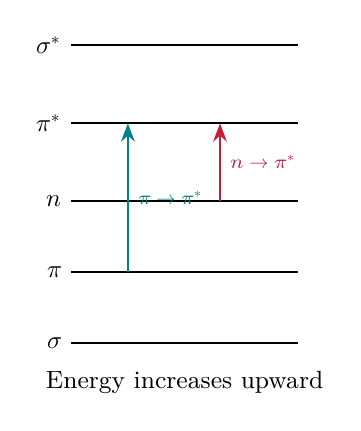
\begin{tikzpicture}[scale=0.9]
  \foreach \y/\lab in {0/$\sigma$,1.0/$\pi$,2.0/$n$,3.1/$\pi^*$,4.2/$\sigma^*$} {
    \draw[thick] (0,\y) -- (3.2,\y);
    \node[left,font=\small] at (0,\y) {\lab};
  }
  \draw[arrow,myteal] (0.8,1.0) -- (0.8,3.1) node[midway,right,font=\scriptsize] {$\pi\rightarrow\pi^*$};
  \draw[arrow,myred] (2.1,2.0) -- (2.1,3.1) node[midway,right,font=\scriptsize] {$n\rightarrow\pi^*$};
  \node[font=\small] at (1.6,-0.55) {Energy increases upward};
\end{tikzpicture}
\end{tcolorbox}

\subsection{Fluorescence and Medical Applications}
Fluorescence occurs when a molecule absorbs light and quickly emits lower-energy light. It is useful in diagnostics, bio-imaging, and detection of trace biomolecules.

\begin{tcolorbox}[tikzbox, title={Jablonski Diagram for Fluorescence}]
\centering
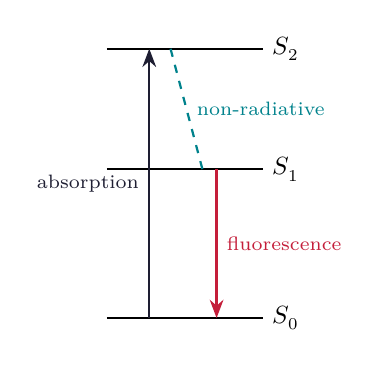
\begin{tikzpicture}[scale=0.9]
  \draw[thick] (0,0) -- (2.2,0) node[right,font=\small] {$S_0$};
  \draw[thick] (0,2.1) -- (2.2,2.1) node[right,font=\small] {$S_1$};
  \draw[thick] (0,3.8) -- (2.2,3.8) node[right,font=\small] {$S_2$};
  \draw[arrow] (0.6,0) -- (0.6,3.8) node[midway,left,font=\scriptsize] {absorption};
  \draw[redarrow] (1.55,2.1) -- (1.55,0) node[midway,right,font=\scriptsize] {fluorescence};
  \draw[thick, dashed, myteal] (0.9,3.8) -- (1.35,2.1) node[midway,right,font=\scriptsize] {non-radiative};
\end{tikzpicture}
\end{tcolorbox}

\subsection{Vibrational and Rotational Spectroscopy}
IR spectroscopy studies molecular vibrations. A vibration is IR active if it changes dipole moment. Rotational spectroscopy is observed mainly for gas-phase polar molecules.

\begin{tcolorbox}[formulabox, title={Vibrational Frequency of a Diatomic Molecule}]
\[
\nu=\frac{1}{2\pi}\sqrt{\frac{k}{\mu}},\qquad
\mu=\frac{m_1m_2}{m_1+m_2}
\]
where $k$ is force constant and $\mu$ is reduced mass.
\end{tcolorbox}

\subsection{NMR, MRI, Surface Characterisation, Diffraction}
NMR detects nuclei in a magnetic field. MRI is a medical imaging application of NMR, mainly using hydrogen nuclei in water and fat. Surface characterisation methods such as XPS, SEM, and AFM help study surface composition and morphology. Diffraction and scattering reveal crystal structure, particle size, and defects.

\begin{tcolorbox}[formulabox, title={Bragg Equation}]
\[
n\lambda=2d\sin\theta
\]
Here $d$ is interplanar spacing and $\theta$ is the Bragg angle.
\end{tcolorbox}

\begin{tcolorbox}[exambox, title={Exam Points}]
\begin{itemize}[leftmargin=*, itemsep=2pt, topsep=2pt]
  \item Mention the energy region: microwave for rotational, IR for vibrational, UV-visible for electronic.
  \item In fluorescence answers, draw the Jablonski diagram.
  \item For NMR/MRI, write the need for non-zero nuclear spin.
  \item For X-ray diffraction, Bragg equation is compulsory.
\end{itemize}
\end{tcolorbox}

% ===============================================================================
\section{Detailed Spectroscopy Notes for Exam Answers}
% ===============================================================================

\subsection{Electromagnetic Spectrum and Type of Transition}
Each spectroscopic method works in a particular energy region. In exam answers, first identify the radiation region, then the molecular transition.

\begin{tabularx}{\linewidth}{|B{3.0cm}|Y|Y|}
\hline
\textbf{Region} & \textbf{Approximate wavelength / frequency} & \textbf{Transition observed} \\
\hline
Radiofrequency & MHz range & Nuclear spin transitions in NMR \\
\hline
Microwave & $1\ \mathrm{mm}$ to $1\ \mathrm{m}$ & Rotational transitions \\
\hline
Infrared & $4000$--$400\ \mathrm{cm^{-1}}$ & Vibrational transitions \\
\hline
Visible / UV & $800$--$200\ \mathrm{nm}$ & Electronic transitions \\
\hline
X-ray & Very short wavelength & Diffraction by crystal planes \\
\hline
\end{tabularx}

\subsection{Beer-Lambert Law in Electronic Spectroscopy}
UV-visible spectroscopy is often used for concentration measurement. If monochromatic light passes through a solution:
\[
A=\log\frac{I_0}{I}
\]
where $I_0$ is incident intensity and $I$ is transmitted intensity.

\begin{tcolorbox}[formulabox, title={Beer-Lambert Law}]
\[
A=\varepsilon c l
\]
where $A$ is absorbance, $\varepsilon$ is molar absorptivity in $\mathrm{L\,mol^{-1}\,cm^{-1}}$, $c$ is concentration in $\mathrm{mol\,L^{-1}}$, and $l$ is path length in cm.
\end{tcolorbox}

\begin{tcolorbox}[examplebox, title={Solved Example: Absorbance}]
If $\varepsilon=2.0\times10^4\ \mathrm{L\,mol^{-1}\,cm^{-1}}$, $c=1.0\times10^{-5}\ \mathrm{mol\,L^{-1}}$, and $l=1\ \mathrm{cm}$:
\[
A=\varepsilon cl=(2.0\times10^4)(1.0\times10^{-5})(1)=0.20
\]
So the solution has absorbance $0.20$.
\end{tcolorbox}

\subsection{IR Spectroscopy: Functional Group Region}
IR spectra are very useful for identifying functional groups. The fingerprint region helps confirm identity, while the functional group region gives quick structural clues.

\begin{tabularx}{\linewidth}{|B{3.2cm}|Y|Y|}
\hline
\textbf{Bond / group} & \textbf{Typical range} & \textbf{Exam identification} \\
\hline
O--H stretch & $3200$--$3600\ \mathrm{cm^{-1}}$ & Broad band for alcohols and acids \\
\hline
N--H stretch & $3300$--$3500\ \mathrm{cm^{-1}}$ & Amine or amide indication \\
\hline
C=O stretch & $1650$--$1800\ \mathrm{cm^{-1}}$ & Strong sharp carbonyl peak \\
\hline
C=C stretch & $1600$--$1680\ \mathrm{cm^{-1}}$ & Alkene or aromatic ring \\
\hline
C--O stretch & $1000$--$1300\ \mathrm{cm^{-1}}$ & Alcohol, ether, ester \\
\hline
\end{tabularx}

\subsection{NMR Chemical Shift and Splitting}
In proton NMR, chemical shift tells the electronic environment. Spin-spin splitting tells the number of neighbouring equivalent protons.

\begin{tcolorbox}[formulabox, title={NMR Splitting Rule}]
If a proton has $n$ equivalent neighbouring protons, its signal is split into:
\[
n+1\ \text{peaks}
\]
The relative intensities approximately follow Pascal's triangle.
\end{tcolorbox}

\begin{tabularx}{\linewidth}{|B{3.0cm}|Y|Y|}
\hline
\textbf{Proton type} & \textbf{Typical chemical shift} & \textbf{Reason} \\
\hline
Alkyl $\mathrm{R-CH_3}$ & $0.8$--$1.5\ \mathrm{ppm}$ & Shielded environment \\
\hline
Near electronegative atom & $3$--$4.5\ \mathrm{ppm}$ & Deshielding by O, N, halogen \\
\hline
Aromatic proton & $6.5$--$8\ \mathrm{ppm}$ & Ring current effect \\
\hline
Aldehydic proton & $9$--$10\ \mathrm{ppm}$ & Strongly deshielded \\
\hline
\end{tabularx}

\subsection{Bragg Law Derivation Idea}
Constructive interference occurs when the path difference between X-rays reflected from successive crystal planes is an integral multiple of wavelength.
\[
\text{Path difference}=AB+BC=2d\sin\theta
\]
For constructive interference:
\[
n\lambda=2d\sin\theta
\]
This equation is used to calculate interplanar spacing $d$ from diffraction angle.

\begin{tcolorbox}[examplebox, title={Solved Example: Crystal Plane Spacing}]
For first-order reflection, $\lambda=1.54\ \text{\AA}$ and $\theta=30^\circ$:
\[
d=\frac{n\lambda}{2\sin\theta}=\frac{1.54}{2\sin30^\circ}
\]
\[
d=\frac{1.54}{1}=1.54\ \text{\AA}
\]
\end{tcolorbox}

\begin{tcolorbox}[masonbox, title={Answer-Writing Pattern for Spectroscopy}]
\begin{enumerate}[leftmargin=*, itemsep=3pt, topsep=2pt]
  \item State the radiation region and energy transition.
  \item Give the selection rule or activity condition.
  \item Draw the transition diagram if possible.
  \item Mention one analytical or medical application.
  \item For numerical questions, write units clearly.
\end{enumerate}
\end{tcolorbox}

\subsection{Rotational Spectroscopy of a Rigid Diatomic Molecule}
For a rigid rotor, rotational energy levels are quantized:
\[
E_J=\frac{h^2}{8\pi^2I}J(J+1),\qquad J=0,1,2,\ldots
\]
where $I=\mu r^2$ is moment of inertia, $\mu$ is reduced mass, and $r$ is bond length.

\begin{tcolorbox}[formulabox, title={Rotational Spectral Lines}]
In wavenumber units:
\[
\bar{\nu}=2B(J+1),\qquad B=\frac{h}{8\pi^2Ic}
\]
Successive lines are equally spaced by:
\[
\Delta\bar{\nu}=2B
\]
\end{tcolorbox}

\begin{tcolorbox}[examplebox, title={Solved Example: Rotational Line Spacing}]
If the rotational constant of a molecule is $B=5\ \mathrm{cm^{-1}}$, then adjacent rotational spectral lines are separated by:
\[
\Delta\bar{\nu}=2B=10\ \mathrm{cm^{-1}}
\]
\end{tcolorbox}

\subsection{Vibrational Spectroscopy and Hooke's Law Model}
A diatomic molecule behaves approximately like two masses connected by a spring. Stronger bonds have larger force constant $k$ and therefore absorb at higher wavenumber.

\begin{tabularx}{\linewidth}{|B{3.2cm}|Y|Y|}
\hline
\textbf{Factor} & \textbf{Effect on frequency} & \textbf{Reason} \\
\hline
Higher force constant & Frequency increases & Bond is stiffer \\
\hline
Higher reduced mass & Frequency decreases & Heavier atoms vibrate more slowly \\
\hline
Hydrogen bonding & O--H/N--H peak becomes broad & Different bond strengths in association \\
\hline
Conjugation near C=O & C=O frequency decreases slightly & Partial single-bond character increases \\
\hline
\end{tabularx}

\subsection{Electronic Spectra: Bathochromic and Hypsochromic Shifts}
Electronic absorption changes when substituents or solvents change the energy gap between molecular orbitals.

\begin{tabularx}{\linewidth}{|B{3.4cm}|Y|Y|}
\hline
\textbf{Term} & \textbf{Meaning} & \textbf{Simple interpretation} \\
\hline
Bathochromic shift & Shift to longer wavelength & Energy gap decreases; red shift \\
\hline
Hypsochromic shift & Shift to shorter wavelength & Energy gap increases; blue shift \\
\hline
Hyperchromic effect & Increase in absorption intensity & More allowed transition or greater conjugation \\
\hline
Hypochromic effect & Decrease in absorption intensity & Less allowed transition or restricted structure \\
\hline
\end{tabularx}

\subsection{Fluorescence Versus Phosphorescence}
Fluorescence and phosphorescence are both emission processes, but their lifetimes and electronic states differ.

\begin{tabularx}{\linewidth}{|B{3cm}|Y|Y|}
\hline
\textbf{Point} & \textbf{Fluorescence} & \textbf{Phosphorescence} \\
\hline
Transition & Singlet to singlet & Triplet to singlet \\
\hline
Lifetime & Very short, about $10^{-9}$--$10^{-7}\ \mathrm{s}$ & Longer, milliseconds to seconds \\
\hline
Spin rule & Spin-allowed & Spin-forbidden, so slow \\
\hline
Observation & Stops quickly when source is removed & May continue after source is removed \\
\hline
\end{tabularx}

\begin{tcolorbox}[masonbox, title={Previous-Year Style Questions}]
\begin{enumerate}[leftmargin=*, itemsep=4pt, topsep=2pt]
  \item Explain selection rules for rotational and vibrational spectroscopy.
  \item Derive the expression for vibrational frequency of a diatomic molecule.
  \item Explain fluorescence with Jablonski diagram and give medical applications.
  \item State Beer-Lambert law and solve a concentration-based numerical.
  \item Derive Bragg law and explain its use in crystal structure determination.
\end{enumerate}
\end{tcolorbox}

\subsection{Short Notes on Surface Characterisation}
Surface characterisation is used to study the outermost layers of solids, thin films, catalysts, sensors and biomaterials. These methods are important in engineering because surface properties often decide corrosion resistance, adhesion, catalytic activity and device performance.

\begin{tabularx}{\linewidth}{|B{3.2cm}|Y|Y|}
\hline
\textbf{Technique} & \textbf{Information obtained} & \textbf{Engineering use} \\
\hline
SEM & Surface morphology and particle shape & Fracture surface, coating quality, microstructure \\
\hline
AFM & Nanometre-scale surface topography & Thin films, MEMS surfaces, biomaterials \\
\hline
XPS & Surface elemental composition and oxidation state & Corrosion films, catalysts, semiconductor surfaces \\
\hline
XRD & Crystal structure and interplanar spacing & Phase identification and crystallinity \\
\hline
\end{tabularx}

\begin{tcolorbox}[examplebox, title={Exam Answer: Why Surface Analysis Matters}]
Bulk composition may remain unchanged while the surface oxidizes, adsorbs impurities or forms a thin passive layer. Therefore surface techniques are needed to understand corrosion, catalysis, coating failure and sensor response.
\end{tcolorbox}
\newpage
\begin{center}
  {\large\bfseries\color{myred} Quick Revision --- Module 2}\\[3pt]
  {\small\color{mydark} Spectroscopic Techniques and Applications $|$ BS-CH101}
\end{center}
\noindent{\color{myred}\rule{\linewidth}{1.2pt}}
\vspace{4pt}

\begin{tcolorbox}[formulabox, title={Key Formulas at a Glance}]
\begin{tabularx}{\linewidth}{|B{4.0cm}|Y|}
\hline
\textbf{Formula / Rule} & \textbf{Meaning} \\
\hline
$\Delta E=h\nu=\displaystyle\frac{hc}{\lambda}$ & Photon energy absorbed or emitted in spectroscopy. \\
\hline
$\Delta J=\pm1$ & Rotational selection rule. \\
\hline
$\Delta v=\pm1$ & Fundamental vibrational transition rule. \\
\hline
$\nu=\displaystyle\frac{1}{2\pi}\sqrt{\displaystyle\frac{k}{\mu}}$ & Diatomic vibrational frequency. \\
\hline
$\mu=\displaystyle\frac{m_1m_2}{m_1+m_2}$ & Reduced mass of a diatomic molecule. \\
\hline
$n\lambda=2d\sin\theta$ & Bragg equation for diffraction. \\
\hline
\end{tabularx}
\end{tcolorbox}

\begin{tcolorbox}[defbox, title={One-Line Definitions}]
\begin{itemize}[leftmargin=*, itemsep=2pt, topsep=2pt]
  \item \textbf{Spectroscopy:} Study of interaction of radiation with matter.
  \item \textbf{Selection rule:} Condition deciding whether a transition is allowed.
  \item \textbf{Chromophore:} Group responsible for UV-visible absorption.
  \item \textbf{Fluorescence:} Fast emission after electronic excitation.
  \item \textbf{IR active vibration:} Vibration causing a change in dipole moment.
  \item \textbf{Chemical shift:} NMR position relative to a reference.
  \item \textbf{Diffraction:} Constructive interference of waves scattered by ordered planes.
\end{itemize}
\end{tcolorbox}

\begin{tcolorbox}[exambox, title={Frequently Asked / Viva Questions}]
\begin{enumerate}[topsep=0pt, label=\textbf{Q\arabic*.}, itemsep=5pt]
  \item \Q{What is spectroscopy?}
    It is the study of absorption, emission, or scattering of radiation by matter.
  \item \Q{Write the relation between energy and wavelength.}
    $\Delta E=hc/\lambda$.
  \item \Q{What is a selection rule?}
    It is a rule that decides whether a spectroscopic transition is allowed.
  \item \Q{Why are rotational spectra shown by polar molecules?}
    Rotation must produce an oscillating dipole moment.
  \item \Q{What is the condition for IR activity?}
    The vibration must change the dipole moment of the molecule.
  \item \Q{What is fluorescence?}
    It is emission of light from an excited singlet state to the ground state.
  \item \Q{Give one medical use of fluorescence.}
    Fluorescent probes are used in bio-imaging and disease diagnostics.
  \item \Q{What is NMR based on?}
    Resonance absorption by nuclei with non-zero spin in a magnetic field.
  \item \Q{How is MRI related to NMR?}
    MRI is an imaging technique based on NMR signals, mainly from hydrogen nuclei.
  \item \Q{State Bragg law.}
    $n\lambda=2d\sin\theta$.
\end{enumerate}
\end{tcolorbox}

\begin{tcolorbox}[tikzbox, title={Summary Reference Table}]
\begin{tabularx}{\linewidth}{|B{3cm}|Y|Y|}
\hline
\textbf{Method} & \textbf{Radiation / signal} & \textbf{Main application} \\
\hline
UV-visible & Electronic transitions & Conjugation and concentration \\
\hline
Fluorescence & Emitted visible light & Medical imaging and trace analysis \\
\hline
IR & Vibrational transitions & Functional group identification \\
\hline
NMR/MRI & Nuclear spin resonance & Structure and medical imaging \\
\hline
XRD & Diffracted X-rays & Crystal structure \\
\hline
\end{tabularx}
\end{tcolorbox}


% -- Module 3 -----------------------------------------------------------------
\modulestart{3}{Intermolecular Forces and Potential Energy Surfaces}

\section{Intermolecular Forces and Potential Energy Surfaces}
% ===============================================================================

\begin{tcolorbox}[defbox]
\textbf{Intermolecular forces} are attractive or repulsive forces between molecules or ions. They are weaker than covalent bonds but strongly affect boiling point, solubility, viscosity, and real-gas behaviour.
\end{tcolorbox}

\subsection{Ionic, Dipole and Van der Waals Interactions}
Ionic interactions are strongest among common non-covalent interactions. Dipole-dipole forces occur between polar molecules. London dispersion forces arise from temporary induced dipoles and exist in all molecules.

\begin{tabularx}{\linewidth}{|B{3.2cm}|Y|Y|}
\hline
\textbf{Interaction} & \textbf{Origin} & \textbf{Example} \\
\hline
Ion-ion & Attraction between full charges & $\mathrm{Na^+}$ and $\mathrm{Cl^-}$ \\
\hline
Ion-dipole & Ion attracts polar molecule & Hydration of $\mathrm{Na^+}$ \\
\hline
Dipole-dipole & Permanent dipoles align & $\mathrm{HCl}$ molecules \\
\hline
London dispersion & Instantaneous induced dipoles & Noble gases, hydrocarbons \\
\hline
Hydrogen bonding & H attached to F, O, or N interacts with lone pair & Water, alcohols \\
\hline
\end{tabularx}

\subsection{Potential Energy Curve}
The potential energy between two particles depends on separation distance. At equilibrium distance $r_e$, attractive and repulsive forces balance and potential energy is minimum.

\begin{tcolorbox}[tikzbox, title={Potential Energy Curve for Intermolecular Interaction}]
\centering
\begin{tikzpicture}[scale=0.92]
  \draw[->, thick] (0,0) -- (7.2,0) node[right] {$r$};
  \draw[->, thick] (0,-2.2) -- (0,2.2) node[above] {$V(r)$};
  \draw[myteal, thick, domain=0.45:6.7, samples=160]
    plot(\x,{1.8*exp(-2.2*\x)-2.4*\x*exp(-1.05*\x)});
  \draw[dashed] (1.32,0) -- (1.32,-1.55);
  \node[font=\small] at (1.32,0.35) {$r_e$};
  \node[font=\small] at (4.6,-1.0) {attraction};
  \node[font=\small] at (1.0,1.5) {repulsion};
\end{tikzpicture}
\end{tcolorbox}

\subsection{Equations of State for Real Gases}
Ideal gas equation assumes no intermolecular force and zero molecular volume. Real gases deviate at high pressure and low temperature.

\begin{tcolorbox}[formulabox, title={Van der Waals Equation}]
\[
\left(P+\frac{a n^2}{V^2}\right)(V-nb)=nRT
\]
where $a$ corrects attractive forces and $b$ corrects finite molecular volume.
\end{tcolorbox}

\subsection{Critical Phenomena}
The critical temperature $T_c$ is the temperature above which a gas cannot be liquefied by pressure alone. At the critical point, liquid and vapour become indistinguishable.

\begin{tcolorbox}[formulabox, title={Critical Constants for a Van der Waals Gas}]
\[
V_c=3nb,\qquad P_c=\frac{a}{27b^2},\qquad T_c=\frac{8a}{27Rb}
\]
\end{tcolorbox}

\begin{tcolorbox}[exambox, title={Exam Points}]
\begin{itemize}[leftmargin=*, itemsep=2pt, topsep=2pt]
  \item Compare intermolecular forces by strength and origin.
  \item Draw the potential energy curve and mark $r_e$ and minimum energy.
  \item For real gases, explain physical meaning of constants $a$ and $b$.
  \item Define critical temperature, pressure, and volume clearly.
\end{itemize}
\end{tcolorbox}

% ===============================================================================
\section{Detailed Notes on Forces, Real Gases and Critical Behaviour}
% ===============================================================================

\subsection{Origin and Strength of Intermolecular Forces}
Intermolecular force strength depends on charge, polarity, polarizability, and molecular shape. Ionic interactions are strong because full charges are involved. Dispersion forces are weak individually but become important for large molecules with many electrons.

\begin{tabularx}{\linewidth}{|B{3.4cm}|Y|Y|}
\hline
\textbf{Force} & \textbf{Approximate strength trend} & \textbf{Property affected} \\
\hline
Ion-ion & Very strong & Melting point of ionic solids \\
\hline
Ion-dipole & Strong & Hydration and solubility of salts \\
\hline
Hydrogen bond & Moderate to strong & Boiling point of water and alcohols \\
\hline
Dipole-dipole & Moderate & Boiling point of polar molecules \\
\hline
London dispersion & Weak to moderate & Liquefaction of non-polar gases \\
\hline
\end{tabularx}

\subsection{Potential Energy and Force Relation}
The force between two particles is related to the potential energy curve by:
\[
F=-\frac{dV}{dr}
\]
At the equilibrium separation $r_e$, potential energy is minimum, so:
\[
\left(\frac{dV}{dr}\right)_{r=r_e}=0,\qquad F=0
\]
For $r<r_e$, repulsive force dominates. For $r>r_e$, attractive force dominates.

\begin{tcolorbox}[examplebox, title={Exam Interpretation of Potential Energy Curve}]
If two molecules are very far apart, $V(r)\approx0$. As they approach, attraction lowers the potential energy. At $r_e$, the most stable separation is reached. If they come closer than $r_e$, electron-cloud repulsion sharply increases energy.
\end{tcolorbox}

\subsection{Lennard-Jones Potential}
A common model for non-bonded interaction is:
\[
V(r)=4\varepsilon\left[\left(\frac{\sigma}{r}\right)^{12}-\left(\frac{\sigma}{r}\right)^6\right]
\]
The $r^{-12}$ term represents short-range repulsion and the $r^{-6}$ term represents London attraction. $\varepsilon$ indicates well depth, i.e. strength of attraction.

\begin{tabularx}{\linewidth}{|B{3cm}|Y|}
\hline
\textbf{Term} & \textbf{Physical meaning} \\
\hline
$\left(\sigma/r\right)^{12}$ & Repulsion due to electron-cloud overlap \\
\hline
$-\left(\sigma/r\right)^6$ & Attractive dispersion interaction \\
\hline
$\varepsilon$ & Depth of potential well; higher value means stronger attraction \\
\hline
$r_e$ & Separation at minimum potential energy \\
\hline
\end{tabularx}

\subsection{Compressibility Factor and Deviation from Ideality}
Deviation from ideal gas behaviour is often measured using compressibility factor:
\[
Z=\frac{PV}{nRT}
\]
For an ideal gas, $Z=1$. For a real gas, $Z<1$ indicates attraction-dominated behaviour and $Z>1$ indicates repulsion or finite-volume dominated behaviour.

\begin{tcolorbox}[tikzbox, title={Compressibility Factor: Qualitative Behaviour}]
\centering
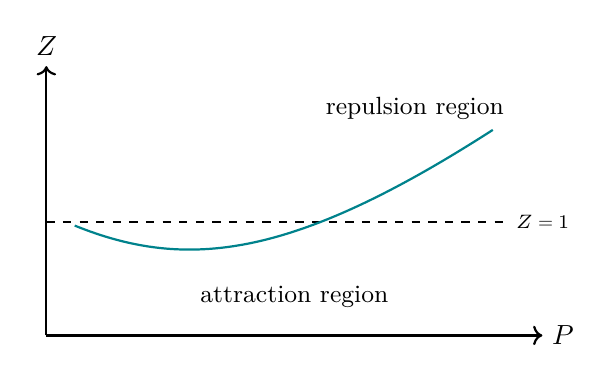
\begin{tikzpicture}[scale=0.9]
  \draw[->, thick] (0,0) -- (7,0) node[right] {$P$};
  \draw[->, thick] (0,0) -- (0,3.8) node[above] {$Z$};
  \draw[dashed] (0,1.6) -- (6.5,1.6) node[right,font=\scriptsize] {$Z=1$};
  \draw[myteal, thick] (0.4,1.55) .. controls (2,0.9) and (3.5,1.1) .. (6.3,2.9);
  \node[font=\small] at (3.5,0.55) {attraction region};
  \node[font=\small] at (5.2,3.2) {repulsion region};
\end{tikzpicture}
\end{tcolorbox}

\subsection{Critical Constants from Van der Waals Equation}
For one mole:
\[
\left(P+\frac{a}{V_m^2}\right)(V_m-b)=RT
\]
At the critical point, the isotherm has a point of inflection:
\[
\left(\frac{\partial P}{\partial V_m}\right)_T=0,\qquad
\left(\frac{\partial^2 P}{\partial V_m^2}\right)_T=0
\]
Solving these conditions gives:
\[
V_c=3b,\qquad P_c=\frac{a}{27b^2},\qquad T_c=\frac{8a}{27Rb}
\]
These relations are often asked as short derivation or formula-based questions.

\begin{tcolorbox}[examplebox, title={Solved Example: Critical Volume}]
If van der Waals constant $b=0.040\ \mathrm{L\,mol^{-1}}$, then:
\[
V_c=3b=3(0.040)=0.120\ \mathrm{L\,mol^{-1}}
\]
\end{tcolorbox}

\begin{tcolorbox}[masonbox, title={How to Score in This Module}]
\begin{itemize}[leftmargin=*, itemsep=2pt, topsep=2pt]
  \item Write force origin, example, and property affected for each intermolecular force.
  \item In potential energy questions, always mark attraction, repulsion, $r_e$, and energy minimum.
  \item For real gases, explain that $a$ corrects pressure and $b$ corrects volume.
  \item Use $Z=PV/nRT$ to discuss positive and negative deviation.
\end{itemize}
\end{tcolorbox}

\subsection{Hydrogen Bonding in Detail}
Hydrogen bonding occurs when hydrogen is covalently bonded to a highly electronegative atom such as F, O, or N and interacts with a lone pair on another electronegative atom.

\begin{tabularx}{\linewidth}{|B{3.3cm}|Y|Y|}
\hline
\textbf{Type} & \textbf{Meaning} & \textbf{Example} \\
\hline
Intermolecular hydrogen bonding & Hydrogen bond between different molecules & Water, alcohols, HF \\
\hline
Intramolecular hydrogen bonding & Hydrogen bond within the same molecule & o-nitrophenol type structures \\
\hline
Strong hydrogen bonding & Shorter and more directional interaction & HF, water network \\
\hline
Weak hydrogen bonding & Longer and less directional interaction & C--H based weak interactions \\
\hline
\end{tabularx}

\begin{tcolorbox}[examplebox, title={Exam Explanation: Boiling Point of Water}]
Water has a much higher boiling point than $\mathrm{H_2S}$ because oxygen is highly electronegative and forms extensive intermolecular hydrogen bonding. More heat is required to break this associated network before molecules escape into vapour phase.
\end{tcolorbox}

\subsection{Corresponding States and Reduced Variables}
The law of corresponding states states that gases behave similarly when compared at the same reduced temperature and reduced pressure.

\begin{tcolorbox}[formulabox, title={Reduced Variables}]
\[
T_r=\frac{T}{T_c},\qquad P_r=\frac{P}{P_c},\qquad V_r=\frac{V}{V_c}
\]
where $T_c$, $P_c$, and $V_c$ are critical constants.
\end{tcolorbox}

\subsection{Boyle Temperature}
At Boyle temperature, a real gas behaves nearly ideally over a considerable pressure range because attractive and repulsive deviations approximately cancel.
\[
Z\approx1
\]
For a van der Waals gas, the Boyle temperature is approximately:
\[
T_B=\frac{a}{Rb}
\]

\begin{tcolorbox}[examplebox, title={Solved Example: Boyle Temperature}]
If $a=1.36\ \mathrm{L^2\,atm\,mol^{-2}}$ and $b=0.0318\ \mathrm{L\,mol^{-1}}$:
\[
T_B=\frac{a}{Rb}=\frac{1.36}{(0.0821)(0.0318)}
\]
\[
T_B\approx521\ \mathrm{K}
\]
\end{tcolorbox}

\subsection{Joule-Thomson Effect}
When a real gas expands through a porous plug from high pressure to low pressure without external work and without heat exchange, its temperature may change. This is called Joule-Thomson effect.

\begin{tcolorbox}[defbox]
\textbf{Inversion temperature:} The temperature at which Joule-Thomson coefficient becomes zero. Below it, gas cools on expansion; above it, gas warms on expansion.
\end{tcolorbox}

\begin{tabularx}{\linewidth}{|B{3.0cm}|Y|Y|}
\hline
\textbf{Condition} & \textbf{Joule-Thomson coefficient} & \textbf{Observation} \\
\hline
$T<T_i$ & Positive & Gas cools on expansion \\
\hline
$T=T_i$ & Zero & No temperature change \\
\hline
$T>T_i$ & Negative & Gas warms on expansion \\
\hline
\end{tabularx}

\subsection{Potential Energy Surface in Chemical Reactions}
A potential energy surface shows how molecular energy changes with geometry. Reactants, products, intermediates, and transition states are represented as regions on the surface.

\begin{tcolorbox}[tikzbox, title={Reaction Path on a Potential Energy Surface}]
\centering
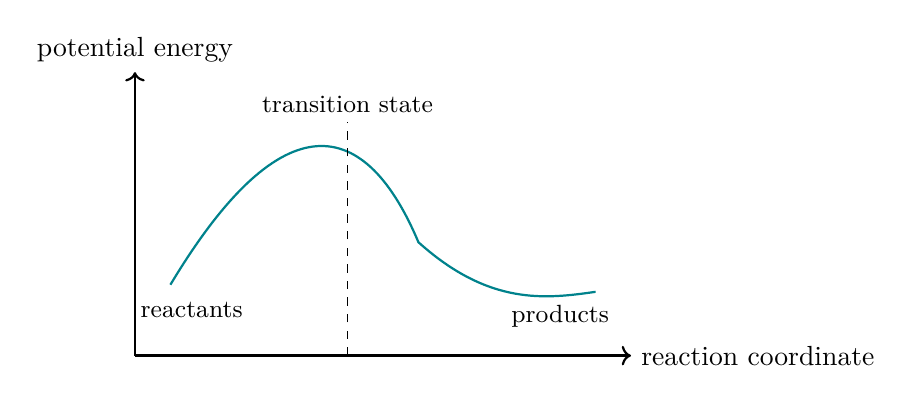
\begin{tikzpicture}[scale=0.9]
  \draw[->, thick] (0,0) -- (7,0) node[right] {reaction coordinate};
  \draw[->, thick] (0,0) -- (0,4) node[above] {potential energy};
  \draw[myteal, thick] (0.5,1.0) .. controls (2,3.5) and (3.2,3.5) .. (4.0,1.6)
    .. controls (5.0,0.7) and (5.8,0.8) .. (6.5,0.9);
  \node[font=\small] at (0.8,0.65) {reactants};
  \node[font=\small] at (3.0,3.55) {transition state};
  \node[font=\small] at (6.0,0.55) {products};
  \draw[dashed] (3.0,0) -- (3.0,3.3);
\end{tikzpicture}
\end{tcolorbox}

\begin{tcolorbox}[masonbox, title={Previous-Year Style Questions}]
\begin{enumerate}[leftmargin=*, itemsep=4pt, topsep=2pt]
  \item Compare ion-dipole, dipole-dipole, hydrogen bonding and dispersion forces.
  \item Explain the potential energy curve for two interacting molecules.
  \item Derive or state critical constants of a van der Waals gas.
  \item Explain compressibility factor and deviation from ideal behaviour.
  \item Write short notes on Joule-Thomson effect and inversion temperature.
\end{enumerate}
\end{tcolorbox}

\subsection{Applications of Intermolecular Forces in Engineering Chemistry}
Intermolecular forces are not only theoretical; they explain important material and chemical behaviour.

\begin{tabularx}{\linewidth}{|B{3.0cm}|Y|Y|}
\hline
\textbf{Application} & \textbf{Force involved} & \textbf{Importance} \\
\hline
Solubility of salts in water & Ion-dipole force & Hydration stabilizes ions in solution \\
\hline
Polymer strength & Dipole interaction and hydrogen bonding & Controls toughness, flexibility and melting range \\
\hline
Adsorption on catalyst & van der Waals and polar interactions & Reactants attach to active surface sites \\
\hline
Boiling point of liquids & Hydrogen bonding and dispersion & Stronger forces increase boiling point \\
\hline
Protein structure & Hydrogen bonding and hydrophobic interaction & Maintains secondary and tertiary structure \\
\hline
\end{tabularx}

\begin{tcolorbox}[examplebox, title={Exam Answer: Like Dissolves Like}]
Polar solvents dissolve ionic and polar solutes because ion-dipole or dipole-dipole interactions compensate for the energy needed to separate solute particles. Non-polar solutes dissolve better in non-polar solvents because dispersion forces are similar in both.
\end{tcolorbox}
\newpage
\begin{center}
  {\large\bfseries\color{myred} Quick Revision --- Module 3}\\[3pt]
  {\small\color{mydark} Intermolecular Forces and Potential Energy Surfaces $|$ BS-CH101}
\end{center}
\noindent{\color{myred}\rule{\linewidth}{1.2pt}}
\vspace{4pt}

\begin{tcolorbox}[formulabox, title={Key Formulas at a Glance}]
\begin{tabularx}{\linewidth}{|B{4.0cm}|Y|}
\hline
\textbf{Formula / Rule} & \textbf{Meaning} \\
\hline
$F=-\displaystyle\frac{dV}{dr}$ & Force is negative gradient of potential energy. \\
\hline
$PV=nRT$ & Ideal gas equation. \\
\hline
$\left(P+\displaystyle\frac{an^2}{V^2}\right)(V-nb)=nRT$ & Van der Waals real-gas equation. \\
\hline
$V_c=3nb$ & Critical volume for van der Waals gas. \\
\hline
$P_c=\displaystyle\frac{a}{27b^2}$ & Critical pressure for one mole form. \\
\hline
$T_c=\displaystyle\frac{8a}{27Rb}$ & Critical temperature for one mole form. \\
\hline
\end{tabularx}
\end{tcolorbox}

\begin{tcolorbox}[defbox, title={One-Line Definitions}]
\begin{itemize}[leftmargin=*, itemsep=2pt, topsep=2pt]
  \item \textbf{Intermolecular force:} Force acting between molecules or ions.
  \item \textbf{Dipole moment:} Product of charge and separation in a polar molecule.
  \item \textbf{Hydrogen bond:} Strong dipole interaction involving H bonded to F, O, or N.
  \item \textbf{Potential energy surface:} Energy variation with molecular geometry.
  \item \textbf{Real gas:} Gas that deviates from ideal behaviour due to volume and attraction.
  \item \textbf{Critical temperature:} Highest temperature at which gas can be liquefied by pressure.
\end{itemize}
\end{tcolorbox}

\begin{tcolorbox}[exambox, title={Frequently Asked / Viva Questions}]
\begin{enumerate}[topsep=0pt, label=\textbf{Q\arabic*.}, itemsep=5pt]
  \item \Q{What are intermolecular forces?}
    Forces of attraction or repulsion acting between separate molecules or ions.
  \item \Q{Arrange common forces in increasing strength.}
    London dispersion $<$ dipole-dipole $<$ hydrogen bonding $<$ ion-dipole $<$ ion-ion.
  \item \Q{Why does boiling point increase with stronger intermolecular force?}
    More energy is needed to separate molecules into vapour.
  \item \Q{What is equilibrium separation in a potential energy curve?}
    It is the distance where potential energy is minimum and net force is zero.
  \item \Q{What causes repulsion at very small distance?}
    Overlap of electron clouds and nuclear repulsion.
  \item \Q{Why do real gases deviate from ideal behaviour?}
    Molecules have finite volume and attractive forces.
  \item \Q{What is the role of $a$ in van der Waals equation?}
    It corrects pressure for intermolecular attraction.
  \item \Q{What is the role of $b$ in van der Waals equation?}
    It corrects volume for finite molecular size.
  \item \Q{Define critical point.}
    The point at which liquid and vapour phases become indistinguishable.
  \item \Q{What is critical temperature?}
    The highest temperature above which gas cannot be liquefied by pressure alone.
\end{enumerate}
\end{tcolorbox}

\begin{tcolorbox}[tikzbox, title={Summary Reference Table}]
\begin{tabularx}{\linewidth}{|B{3.2cm}|Y|Y|}
\hline
\textbf{Concept} & \textbf{Meaning} & \textbf{Must write in exam} \\
\hline
Intermolecular forces & Non-covalent forces between species & Strength order and examples \\
\hline
Potential curve & Energy versus separation & Minimum at $r_e$ \\
\hline
Real gas & Non-ideal gas & Van der Waals correction terms \\
\hline
Critical point & End point of liquid-vapour boundary & $T_c$, $P_c$, $V_c$ definitions \\
\hline
\end{tabularx}
\end{tcolorbox}


% -- Module 4 -----------------------------------------------------------------
\modulestart{4}{Free Energy and Chemical Equilibria}

\section{Free Energy and Chemical Equilibria}
% ===============================================================================

\begin{tcolorbox}[defbox]
\textbf{Gibbs free energy} is the thermodynamic function that predicts spontaneity at constant temperature and pressure. A process is spontaneous when $\Delta G<0$.
\end{tcolorbox}

\subsection{First and Second Laws of Thermodynamics}
The first law states conservation of energy. The second law states that total entropy of the universe increases for a spontaneous process.

\begin{tcolorbox}[formulabox, title={Thermodynamic Functions}]
\[
\Delta U=q+w,\qquad \Delta H=\Delta U+\Delta(PV)
\]
\[
\Delta G=\Delta H-T\Delta S
\]
At constant temperature and pressure, $\Delta G<0$ means spontaneous, $\Delta G=0$ means equilibrium, and $\Delta G>0$ means non-spontaneous.
\end{tcolorbox}

\subsection{Entropy and Free Energy Estimation}
Entropy measures dispersal of energy. For a reversible process,
\[
\Delta S=\int\frac{\delta q_{\mathrm{rev}}}{T}
\]
Free energy change combines enthalpy and entropy and is useful because it directly predicts useful work and equilibrium direction.

\subsection{Free Energy and Equilibrium Constant}
For a reaction at non-standard condition,
\[
\Delta G=\Delta G^\circ+RT\ln Q
\]
At equilibrium, $\Delta G=0$ and $Q=K$.

\begin{tcolorbox}[formulabox, title={Relation Between Free Energy and Equilibrium Constant}]
\[
\Delta G^\circ=-RT\ln K=-2.303RT\log K
\]
\end{tcolorbox}

\subsection{Cell Potential and Nernst Equation}
Electrochemical cell work is linked with free energy.

\begin{tcolorbox}[formulabox, title={Electrochemical Free Energy}]
\[
\Delta G=-nFE,\qquad \Delta G^\circ=-nFE^\circ
\]
\[
E=E^\circ-\frac{RT}{nF}\ln Q
\]
At $298\ \mathrm{K}$:
\[
E=E^\circ-\frac{0.0591}{n}\log Q
\]
\end{tcolorbox}

\begin{tcolorbox}[tikzbox, title={Galvanic Cell and Electron Flow}]
\centering
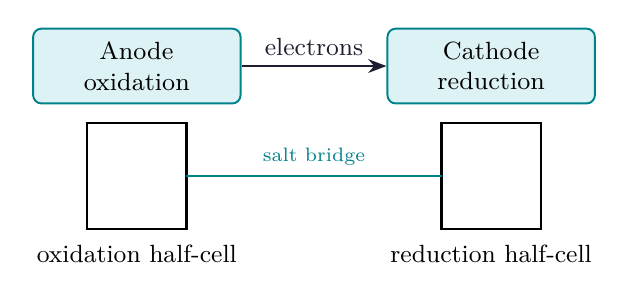
\begin{tikzpicture}[scale=0.9]
  \node[block] (an) at (0,0) {Anode\\oxidation};
  \node[block] (ca) at (5,0) {Cathode\\reduction};
  \draw[arrow] (an) -- node[above,font=\small] {electrons} (ca);
  \draw[thick] (-0.7,-0.8) rectangle (0.7,-2.3);
  \draw[thick] (4.3,-0.8) rectangle (5.7,-2.3);
  \draw[thick,myteal] (0.7,-1.55) -- (4.3,-1.55) node[midway,above,font=\scriptsize] {salt bridge};
  \node[font=\small] at (0,-2.65) {oxidation half-cell};
  \node[font=\small] at (5,-2.65) {reduction half-cell};
\end{tikzpicture}
\end{tcolorbox}

\subsection{Acid-Base, Redox and Solubility Equilibria}
The same free-energy idea applies to acid-base ionization, redox reactions, and precipitation.

\begin{tabularx}{\linewidth}{|B{3.2cm}|Y|Y|}
\hline
\textbf{Equilibrium} & \textbf{Constant} & \textbf{Use} \\
\hline
Acid-base & $K_a$, $K_b$ & pH and strength of acid/base \\
\hline
Redox & $E^\circ$, $K$ & Feasibility of electron transfer \\
\hline
Solubility & $K_{sp}$ & Precipitation and ionic product \\
\hline
\end{tabularx}

\subsection{Water Chemistry, Corrosion and Ellingham Diagram}
Water chemistry includes hardness, alkalinity, pH, and dissolved oxygen. Corrosion is an electrochemical oxidation of metal. Ellingham diagrams plot $\Delta G^\circ$ versus temperature and help choose reducing agents in metallurgy.

\begin{tcolorbox}[tikzbox, title={Ellingham Diagram Concept}]
\centering
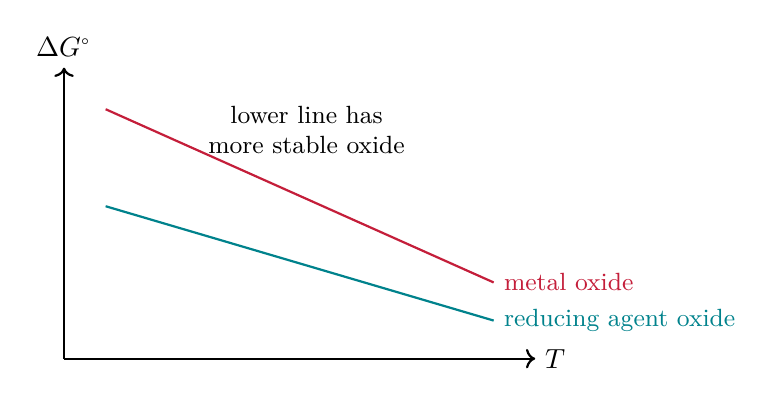
\begin{tikzpicture}[scale=0.88]
  \draw[->, thick] (0,0) -- (6.8,0) node[right] {$T$};
  \draw[->, thick] (0,0) -- (0,4.2) node[above] {$\Delta G^\circ$};
  \draw[myred, thick] (0.6,3.6) -- (6.2,1.1) node[right,font=\small] {metal oxide};
  \draw[myteal, thick] (0.6,2.2) -- (6.2,0.55) node[right,font=\small] {reducing agent oxide};
  \node[font=\small, align=center] at (3.5,3.3) {lower line has\\more stable oxide};
\end{tikzpicture}
\end{tcolorbox}

\begin{tcolorbox}[exambox, title={Exam Points}]
\begin{itemize}[leftmargin=*, itemsep=2pt, topsep=2pt]
  \item Always state sign of $\Delta G$ for spontaneity.
  \item For equilibrium questions, start from $\Delta G=\Delta G^\circ+RT\ln Q$.
  \item For electrochemistry, connect $\Delta G$, $E$, and Nernst equation.
  \item For Ellingham diagrams, lower line means more stable oxide.
\end{itemize}
\end{tcolorbox}

% ===============================================================================
\section{Derivations, Numericals and Engineering Applications}
% ===============================================================================

\subsection{Deriving the Equilibrium Relation}
For any reaction:
\[
\Delta G=\Delta G^\circ+RT\ln Q
\]
At equilibrium, the reaction has no net driving force, so:
\[
\Delta G=0,\qquad Q=K
\]
Therefore:
\[
0=\Delta G^\circ+RT\ln K
\]
\[
\Delta G^\circ=-RT\ln K
\]
Using $\ln K=2.303\log K$:
\[
\Delta G^\circ=-2.303RT\log K
\]

\begin{tcolorbox}[examplebox, title={Solved Example: Equilibrium Constant from Free Energy}]
At $298\ \mathrm{K}$, suppose $\Delta G^\circ=-11.4\ \mathrm{kJ\,mol^{-1}}$.
\[
\log K=\frac{-\Delta G^\circ}{2.303RT}
\]
\[
\log K=\frac{11400}{2.303(8.314)(298)}\approx2.00
\]
\[
K\approx10^2=100
\]
Since $K>1$, products are favoured.
\end{tcolorbox}

\subsection{Entropy Change for Common Processes}
Entropy increases when randomness, volume, or number of gas molecules increases.

\begin{tabularx}{\linewidth}{|B{3.5cm}|Y|Y|}
\hline
\textbf{Process} & \textbf{Entropy change} & \textbf{Reason} \\
\hline
Melting of solid & Positive & Liquid has more molecular freedom \\
\hline
Vaporization & Strongly positive & Gas has much greater randomness \\
\hline
Compression of gas & Negative & Accessible volume decreases \\
\hline
Dissolution of salt & Usually positive & Ions disperse in solution \\
\hline
Crystallization & Negative & Ordered solid forms \\
\hline
\end{tabularx}

\subsection{Nernst Equation Derivation from Free Energy}
Electrical work from a cell is:
\[
\Delta G=-nFE
\]
At standard condition:
\[
\Delta G^\circ=-nFE^\circ
\]
Substitute both in:
\[
\Delta G=\Delta G^\circ+RT\ln Q
\]
\[
-nFE=-nFE^\circ+RT\ln Q
\]
Dividing by $-nF$:
\[
E=E^\circ-\frac{RT}{nF}\ln Q
\]
At $298\ \mathrm{K}$:
\[
E=E^\circ-\frac{0.0591}{n}\log Q
\]

\begin{tcolorbox}[examplebox, title={Solved Example: Cell Potential}]
For a cell with $E^\circ=1.10\ \mathrm{V}$, $n=2$, and $Q=10$:
\[
E=1.10-\frac{0.0591}{2}\log 10
\]
\[
E=1.10-0.02955=1.07045\ \mathrm{V}
\]
\end{tcolorbox}

\subsection{Water Hardness and Boiler Problems}
Hard water contains dissolved calcium and magnesium salts. Temporary hardness is due to bicarbonates; permanent hardness is due to chlorides and sulphates.

\begin{tabularx}{\linewidth}{|B{3.2cm}|Y|Y|}
\hline
\textbf{Problem} & \textbf{Cause} & \textbf{Effect in engineering systems} \\
\hline
Scale formation & Deposition of salts like $\mathrm{CaCO_3}$ & Poor heat transfer and tube overheating \\
\hline
Sludge formation & Loose precipitates in boiler water & Choking and reduced efficiency \\
\hline
Priming & Carryover of water droplets with steam & Wet steam and turbine damage \\
\hline
Foaming & Stable bubbles due to impurities & Irregular boiler operation \\
\hline
Caustic embrittlement & Concentrated alkali in cracks & Boiler metal failure \\
\hline
\end{tabularx}

\subsection{Electrochemical Corrosion Mechanism}
In iron corrosion, anodic and cathodic regions form on the metal surface.

\begin{tcolorbox}[formulabox, title={Rusting Half-Reactions}]
\[
\text{Anode:}\qquad \mathrm{Fe\rightarrow Fe^{2+}+2e^-}
\]
\[
\text{Cathode:}\qquad \mathrm{O_2+2H_2O+4e^-\rightarrow4OH^-}
\]
\[
\mathrm{Fe^{2+}+2OH^-\rightarrow Fe(OH)_2}
\]
Further oxidation gives hydrated ferric oxide, commonly called rust.
\end{tcolorbox}

\subsection{Ellingham Diagram: Reduction Rule}
In metallurgy, a metal oxide can be reduced by an element whose oxide line lies below it in the Ellingham diagram. This means the reducing agent forms a more stable oxide and makes the overall $\Delta G^\circ$ negative.

\begin{tcolorbox}[masonbox, title={Answer-Writing Pattern for Ellingham Problems}]
\begin{enumerate}[leftmargin=*, itemsep=3pt, topsep=2pt]
  \item Identify the oxide to be reduced.
  \item Locate its $\Delta G^\circ$ line at the given temperature.
  \item Find a reducing agent whose oxide line is lower.
  \item State that the net free energy change becomes negative.
\end{enumerate}
\end{tcolorbox}

\subsection{Temperature Dependence of Spontaneity}
The sign of $\Delta G=\Delta H-T\Delta S$ depends on both enthalpy and entropy. This table is a common 5-mark answer.

\begin{tabularx}{\linewidth}{|B{3cm}|Y|Y|}
\hline
\textbf{Case} & \textbf{Sign condition} & \textbf{Spontaneity} \\
\hline
Exothermic, entropy increases & $\Delta H<0,\ \Delta S>0$ & Spontaneous at all temperatures \\
\hline
Endothermic, entropy decreases & $\Delta H>0,\ \Delta S<0$ & Non-spontaneous at all temperatures \\
\hline
Exothermic, entropy decreases & $\Delta H<0,\ \Delta S<0$ & Spontaneous at low temperature \\
\hline
Endothermic, entropy increases & $\Delta H>0,\ \Delta S>0$ & Spontaneous at high temperature \\
\hline
\end{tabularx}

\begin{tcolorbox}[examplebox, title={Solved Example: Temperature of Spontaneity}]
For a reaction, $\Delta H=40\ \mathrm{kJ\,mol^{-1}}$ and $\Delta S=100\ \mathrm{J\,mol^{-1}\,K^{-1}}$.
Convert entropy:
\[
\Delta S=0.100\ \mathrm{kJ\,mol^{-1}\,K^{-1}}
\]
At equilibrium, $\Delta G=0$:
\[
T=\frac{\Delta H}{\Delta S}=\frac{40}{0.100}=400\ \mathrm{K}
\]
Since both $\Delta H$ and $\Delta S$ are positive, the reaction is spontaneous above $400\ \mathrm{K}$.
\end{tcolorbox}

\subsection{pH, Acid Dissociation and Buffer Idea}
For a weak acid:
\[
\mathrm{HA\rightleftharpoons H^+ + A^-}
\]
\[
K_a=\frac{[\mathrm{H^+}][\mathrm{A^-}]}{[\mathrm{HA}]}
\]
For a buffer made of weak acid and its salt:
\[
\mathrm{pH}=pK_a+\log\frac{[\mathrm{salt}]}{[\mathrm{acid}]}
\]

\begin{tcolorbox}[examplebox, title={Solved Example: Buffer pH}]
If $pK_a=4.75$, $[\mathrm{salt}]=0.20\ \mathrm{M}$ and $[\mathrm{acid}]=0.10\ \mathrm{M}$:
\[
\mathrm{pH}=4.75+\log\frac{0.20}{0.10}
\]
\[
\mathrm{pH}=4.75+\log2=4.75+0.301=5.051
\]
\end{tcolorbox}

\subsection{Solubility Product and Common Ion Effect}
For a sparingly soluble salt $\mathrm{AB}$:
\[
\mathrm{AB(s)\rightleftharpoons A^+ + B^-}
\]
\[
K_{sp}=[\mathrm{A^+}][\mathrm{B^-}]
\]
Precipitation occurs when ionic product exceeds $K_{sp}$.

\begin{tabularx}{\linewidth}{|B{3.2cm}|Y|Y|}
\hline
\textbf{Condition} & \textbf{Meaning} & \textbf{Observation} \\
\hline
Ionic product $<K_{sp}$ & Unsaturated solution & No precipitation \\
\hline
Ionic product $=K_{sp}$ & Saturated solution & Equilibrium \\
\hline
Ionic product $>K_{sp}$ & Supersaturated with respect to salt & Precipitation occurs \\
\hline
\end{tabularx}

\subsection{Corrosion Prevention Methods}
Corrosion can be reduced by blocking contact with environment or by making the metal cathodic.

\begin{tabularx}{\linewidth}{|B{3.2cm}|Y|Y|}
\hline
\textbf{Method} & \textbf{Principle} & \textbf{Example} \\
\hline
Painting / coating & Barrier between metal and environment & Paint, oil, polymer coating \\
\hline
Galvanization & Zinc corrodes sacrificially before iron & Zn-coated iron sheets \\
\hline
Cathodic protection & Metal to be protected is made cathode & Pipelines, ship hulls \\
\hline
Alloying & Forms corrosion-resistant surface film & Stainless steel \\
\hline
Inhibitors & Reduce anodic or cathodic reaction rate & Boiler-water additives \\
\hline
\end{tabularx}

\begin{tcolorbox}[masonbox, title={Previous-Year Style Questions}]
\begin{enumerate}[leftmargin=*, itemsep=4pt, topsep=2pt]
  \item Derive $\Delta G^\circ=-RT\ln K$ and explain its significance.
  \item Derive Nernst equation and solve a cell-potential numerical.
  \item Explain water hardness, scale formation and boiler troubles.
  \item Describe electrochemical corrosion of iron and prevention methods.
  \item Explain Ellingham diagram and its use in metallurgy.
\end{enumerate}
\end{tcolorbox}
\newpage
\begin{center}
  {\large\bfseries\color{myred} Quick Revision --- Module 4}\\[3pt]
  {\small\color{mydark} Free Energy and Chemical Equilibria $|$ BS-CH101}
\end{center}
\noindent{\color{myred}\rule{\linewidth}{1.2pt}}
\vspace{4pt}

\begin{tcolorbox}[formulabox, title={Key Formulas at a Glance}]
\begin{tabularx}{\linewidth}{|B{4.0cm}|Y|}
\hline
\textbf{Formula / Rule} & \textbf{Meaning} \\
\hline
$\Delta U=q+w$ & First law of thermodynamics. \\
\hline
$\Delta G=\Delta H-T\Delta S$ & Gibbs free energy relation. \\
\hline
$\Delta G=\Delta G^\circ+RT\ln Q$ & Free energy at non-standard condition. \\
\hline
$\Delta G^\circ=-RT\ln K$ & Relation between free energy and equilibrium constant. \\
\hline
$\Delta G=-nFE$ & Cell free energy and cell potential. \\
\hline
$E=E^\circ-\displaystyle\frac{RT}{nF}\ln Q$ & Nernst equation. \\
\hline
$K_{sp}=[\mathrm{M}^{m+}]^n[\mathrm{X}^{n-}]^m$ & Solubility product expression. \\
\hline
\end{tabularx}
\end{tcolorbox}

\begin{tcolorbox}[defbox, title={One-Line Definitions}]
\begin{itemize}[leftmargin=*, itemsep=2pt, topsep=2pt]
  \item \textbf{Entropy:} Measure of energy dispersal or randomness.
  \item \textbf{Gibbs free energy:} Energy available for useful work at constant temperature and pressure.
  \item \textbf{Equilibrium constant:} Ratio of product and reactant activities at equilibrium.
  \item \textbf{Nernst equation:} Relation between electrode potential and concentration.
  \item \textbf{Corrosion:} Electrochemical deterioration of a metal.
  \item \textbf{Ellingham diagram:} Plot of $\Delta G^\circ$ for oxide formation versus temperature.
\end{itemize}
\end{tcolorbox}

\begin{tcolorbox}[exambox, title={Frequently Asked / Viva Questions}]
\begin{enumerate}[topsep=0pt, label=\textbf{Q\arabic*.}, itemsep=5pt]
  \item \Q{State the first law of thermodynamics.}
    Energy cannot be created or destroyed; $\Delta U=q+w$.
  \item \Q{What is the criterion of spontaneity using Gibbs free energy?}
    $\Delta G<0$ spontaneous, $\Delta G=0$ equilibrium, $\Delta G>0$ non-spontaneous.
  \item \Q{Write Gibbs free energy equation.}
    $\Delta G=\Delta H-T\Delta S$.
  \item \Q{Relate $\Delta G^\circ$ and equilibrium constant.}
    $\Delta G^\circ=-RT\ln K$.
  \item \Q{How is cell emf related to free energy?}
    $\Delta G=-nFE$.
  \item \Q{State the Nernst equation at 298 K.}
    $E=E^\circ-(0.0591/n)\log Q$.
  \item \Q{What is solubility product?}
    It is the product of ion concentrations in a saturated solution, each raised to stoichiometric power.
  \item \Q{Why does corrosion occur electrochemically?}
    Metal oxidation and reduction of oxygen or hydrogen occur at different surface sites.
  \item \Q{What does an Ellingham diagram show?}
    It shows temperature dependence of standard free energy of oxide formation.
  \item \Q{How is a reducing agent selected from Ellingham diagram?}
    A reducing agent whose oxide line lies below the metal oxide line can reduce that oxide.
\end{enumerate}
\end{tcolorbox}

\begin{tcolorbox}[tikzbox, title={Summary Reference Table}]
\begin{tabularx}{\linewidth}{|B{3cm}|Y|Y|}
\hline
\textbf{Area} & \textbf{Key relation} & \textbf{Exam focus} \\
\hline
Thermodynamics & $\Delta G=\Delta H-T\Delta S$ & Spontaneity and equilibrium \\
\hline
Chemical equilibrium & $\Delta G^\circ=-RT\ln K$ & Direction and extent of reaction \\
\hline
Electrochemistry & $\Delta G=-nFE$ & Cell potential and Nernst equation \\
\hline
Metallurgy & Ellingham diagram & Reduction feasibility \\
\hline
\end{tabularx}
\end{tcolorbox}


% -- Module 5 -----------------------------------------------------------------
\modulestart{5}{Periodic Properties}

\section{Periodic Properties}
% ===============================================================================

\begin{tcolorbox}[defbox]
\textbf{Periodic properties} are atomic and chemical properties that vary systematically with atomic number due to effective nuclear charge, shielding, and electronic configuration.
\end{tcolorbox}

\subsection{Effective Nuclear Charge and Shielding}
Outer electrons do not experience the full nuclear charge because inner electrons shield them. Effective nuclear charge is:

\begin{tcolorbox}[formulabox, title={Effective Nuclear Charge}]
\[
Z_{\mathrm{eff}}=Z-\sigma
\]
where $Z$ is nuclear charge and $\sigma$ is shielding constant.
\end{tcolorbox}

\subsection{Penetration and Orbital Energy}
For the same principal shell, penetration order is:
\[
s>p>d>f
\]
More penetrating orbitals experience higher $Z_{\mathrm{eff}}$ and lower energy. Therefore in multi-electron atoms:
\[
E(ns)<E(np)<E(nd)<E(nf)
\]

\begin{tcolorbox}[tikzbox, title={Penetration and Energy Order}]
\centering
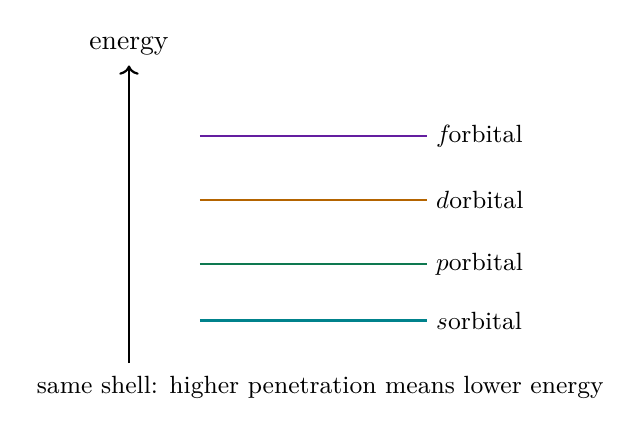
\begin{tikzpicture}[scale=0.9]
  \draw[->, thick] (0,0) -- (0,4.2) node[above] {energy};
  \foreach \y/\lab/\col in {0.6/$s$/myteal,1.4/$p$/mygreen,2.3/$d$/myamber,3.2/$f$/mypurple} {
    \draw[thick,\col] (1,\y) -- (4.2,\y);
    \node[right,font=\small] at (4.2,\y) {\lab orbital};
  }
  \node[font=\small, align=center] at (2.7,-0.35) {same shell: higher penetration means lower energy};
\end{tikzpicture}
\end{tcolorbox}

\subsection{Atomic Size, Ionization Energy, Electron Affinity and Electronegativity}
Across a period, $Z_{\mathrm{eff}}$ increases, so atomic size decreases and ionization energy generally increases. Down a group, new shells are added, so atomic size increases and ionization energy decreases.

\begin{tabularx}{\linewidth}{|B{3.2cm}|Y|Y|}
\hline
\textbf{Property} & \textbf{Across period} & \textbf{Down group} \\
\hline
Atomic radius & Decreases & Increases \\
\hline
Ionization energy & Generally increases & Decreases \\
\hline
Electron affinity & Becomes more negative generally & Less negative generally \\
\hline
Electronegativity & Increases & Decreases \\
\hline
Metallic character & Decreases & Increases \\
\hline
\end{tabularx}

\subsection{Polarizability, Oxidation States and Coordination}
Polarizability increases with size and diffuse electron cloud. Oxidation state depends on valence electron configuration. Coordination number and geometry depend on metal ion size, ligand size, and electron count.

\begin{tabularx}{\linewidth}{|B{2.8cm}|Y|Y|}
\hline
\textbf{Coordination number} & \textbf{Common geometry} & \textbf{Example type} \\
\hline
2 & Linear & $\mathrm{[Ag(NH_3)_2]^+}$ \\
\hline
4 & Tetrahedral or square planar & $\mathrm{[Ni(CN)_4]^{2-}}$ \\
\hline
6 & Octahedral & $\mathrm{[Fe(CN)_6]^{3-}}$ \\
\hline
\end{tabularx}

\subsection{Hard and Soft Acids and Bases}
HSAB principle says hard acids prefer hard bases and soft acids prefer soft bases.

\begin{tcolorbox}[defbox]
\textbf{Hard species} are small, highly charged, and weakly polarizable. \textbf{Soft species} are larger, lower charged, and highly polarizable.
\end{tcolorbox}

\subsection{Molecular Geometries}
VSEPR theory predicts geometry from electron-pair repulsion around the central atom.

\begin{tcolorbox}[tikzbox, title={Common VSEPR Shapes}]
\centering
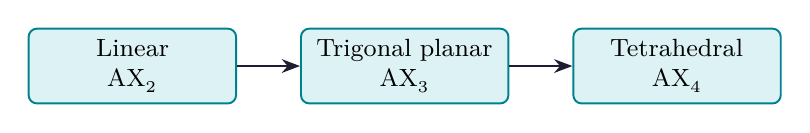
\begin{tikzpicture}[node distance=0.8cm and 0.8cm]
  \node[block] (lin) {Linear\\$\mathrm{AX_2}$};
  \node[block, right=of lin] (tri) {Trigonal planar\\$\mathrm{AX_3}$};
  \node[block, right=of tri] (tet) {Tetrahedral\\$\mathrm{AX_4}$};
  \draw[arrow] (lin) -- (tri);
  \draw[arrow] (tri) -- (tet);
\end{tikzpicture}
\end{tcolorbox}

\begin{tcolorbox}[exambox, title={Exam Points}]
\begin{itemize}[leftmargin=*, itemsep=2pt, topsep=2pt]
  \item Explain periodic trends using $Z_{\mathrm{eff}}$, shielding, and shell number.
  \item For orbital energy, mention penetration order $s>p>d>f$.
  \item HSAB questions need definition plus examples.
  \item Geometry questions should mention electron pairs before shape.
\end{itemize}
\end{tcolorbox}

% ===============================================================================
\section{Detailed Periodic Trend Analysis}
% ===============================================================================

\subsection{Shielding Order and Slater-Type Reasoning}
Shielding is not equal for all orbitals. Inner-shell electrons shield strongly, while electrons in the same shell shield only partially. Poor shielding by $d$ and $f$ electrons explains many irregular periodic trends.

\begin{tabularx}{\linewidth}{|B{3.2cm}|Y|Y|}
\hline
\textbf{Electron type} & \textbf{Shielding ability} & \textbf{Consequence} \\
\hline
$s$ electron & Strong penetration and good shielding & Feels high $Z_{\mathrm{eff}}$ \\
\hline
$p$ electron & Moderate shielding & Higher energy than same-shell $s$ \\
\hline
$d$ electron & Poor shielding & Causes transition-series contraction \\
\hline
$f$ electron & Very poor shielding & Causes lanthanide contraction \\
\hline
\end{tabularx}

\subsection{Successive Ionization Energies}
Successive ionization energies always increase because after removal of one electron, the remaining electrons are held more strongly by the positive ion.
\[
\mathrm{IE_1<IE_2<IE_3<\cdots}
\]
A sudden jump in ionization energy indicates removal of an electron from an inner shell.

\begin{tcolorbox}[examplebox, title={Solved Example: Identifying Valence Electrons}]
If successive ionization energies show the pattern:
\[
580,\quad 1820,\quad 2750,\quad 11600\ \mathrm{kJ\,mol^{-1}}
\]
the large jump occurs after the third electron. Therefore the atom has \textbf{three valence electrons}.
\end{tcolorbox}

\subsection{Diagonal Relationship}
Some second-period elements resemble third-period elements diagonally placed in the periodic table. Examples include Li--Mg, Be--Al, and B--Si. This occurs because size and charge density become comparable.

\begin{tabularx}{\linewidth}{|B{3cm}|Y|Y|}
\hline
\textbf{Pair} & \textbf{Common similarities} & \textbf{Reason} \\
\hline
Li and Mg & Form nitrides; carbonates decompose on heating & Similar charge density \\
\hline
Be and Al & Amphoteric oxides and covalent halides & Small size and high polarizing power \\
\hline
B and Si & Covalent compounds and acidic oxides & Similar electronegativity trend \\
\hline
\end{tabularx}

\subsection{Oxidation States and Inert Pair Effect}
For heavier $p$-block elements, the outer $ns^2$ electron pair becomes less available for bonding. This is called inert pair effect. It stabilizes lower oxidation states.

\begin{tcolorbox}[defbox]
\textbf{Inert pair effect:} Reluctance of the outermost $ns^2$ electron pair of heavier elements to participate in bonding.
\end{tcolorbox}

\begin{tabularx}{\linewidth}{|B{3cm}|Y|Y|}
\hline
\textbf{Group} & \textbf{Higher oxidation state} & \textbf{Lower oxidation state stabilized down group} \\
\hline
Group 13 & $+3$ & $+1$ in Tl \\
\hline
Group 14 & $+4$ & $+2$ in Pb \\
\hline
Group 15 & $+5$ & $+3$ in Bi \\
\hline
\end{tabularx}

\subsection{HSAB Applications}
HSAB theory predicts stability of complexes and salts. Hard-hard and soft-soft combinations are more stable than hard-soft combinations.

\begin{tabularx}{\linewidth}{|B{3.0cm}|Y|Y|}
\hline
\textbf{Acid / base type} & \textbf{Examples} & \textbf{Preferred partner} \\
\hline
Hard acids & $\mathrm{H^+, Li^+, Al^{3+}, Fe^{3+}}$ & Hard bases \\
\hline
Soft acids & $\mathrm{Ag^+, Hg^{2+}, Pt^{2+}}$ & Soft bases \\
\hline
Hard bases & $\mathrm{F^-, OH^-, H_2O, NH_3}$ & Hard acids \\
\hline
Soft bases & $\mathrm{I^-, S^{2-}, CO, PR_3}$ & Soft acids \\
\hline
\end{tabularx}

\begin{tcolorbox}[examplebox, title={Solved Example: HSAB Prediction}]
$\mathrm{Ag^+}$ is a soft acid. Between $\mathrm{F^-}$ and $\mathrm{I^-}$, iodide is softer. Therefore $\mathrm{AgI}$ is more stable and less soluble than expected from simple charge arguments.
\end{tcolorbox}

\subsection{VSEPR Shapes and Lone Pair Effect}
Lone pairs repel more strongly than bond pairs. The repulsion order is:
\[
\text{lone pair-lone pair}>\text{lone pair-bond pair}>\text{bond pair-bond pair}
\]

\begin{tabularx}{\linewidth}{|B{2.8cm}|Y|Y|}
\hline
\textbf{Molecule type} & \textbf{Shape} & \textbf{Example} \\
\hline
$\mathrm{AX_2}$ & Linear & $\mathrm{BeCl_2}$, $\mathrm{CO_2}$ \\
\hline
$\mathrm{AX_3}$ & Trigonal planar & $\mathrm{BF_3}$ \\
\hline
$\mathrm{AX_3E}$ & Trigonal pyramidal & $\mathrm{NH_3}$ \\
\hline
$\mathrm{AX_2E_2}$ & Bent & $\mathrm{H_2O}$ \\
\hline
$\mathrm{AX_4}$ & Tetrahedral & $\mathrm{CH_4}$ \\
\hline
\end{tabularx}

\begin{tcolorbox}[masonbox, title={Periodic Properties: 10-Mark Answer Framework}]
\begin{enumerate}[leftmargin=*, itemsep=3pt, topsep=2pt]
  \item Define the property.
  \item State the trend across period and down group.
  \item Explain trend using $Z_{\mathrm{eff}}$, shielding, and shell size.
  \item Mention exceptions if relevant.
  \item Add one example or application such as HSAB or VSEPR shape.
\end{enumerate}
\end{tcolorbox}

\subsection{Atomic and Ionic Radius: Detailed Trend}
Atomic radius decreases across a period because effective nuclear charge increases while electrons enter the same shell. Down a group, radius increases because a new shell is added.

\begin{tabularx}{\linewidth}{|B{3.2cm}|Y|Y|}
\hline
\textbf{Species compared} & \textbf{Trend} & \textbf{Reason} \\
\hline
Cations vs atoms & Cations are smaller & Electron loss reduces repulsion and may remove outer shell \\
\hline
Anions vs atoms & Anions are larger & Extra electron increases electron-electron repulsion \\
\hline
Isoelectronic species & Radius decreases with increasing nuclear charge & Same electrons pulled by larger $Z$ \\
\hline
\end{tabularx}

\begin{tcolorbox}[examplebox, title={Solved Example: Isoelectronic Radius Order}]
$\mathrm{N^{3-}}$, $\mathrm{O^{2-}}$, $\mathrm{F^-}$, $\mathrm{Na^+}$ and $\mathrm{Mg^{2+}}$ are isoelectronic with 10 electrons.

Higher nuclear charge pulls the same electron cloud more strongly:
\[
\mathrm{N^{3-}>O^{2-}>F^->Na^+>Mg^{2+}}
\]
\end{tcolorbox}

\subsection{Electron Affinity and Exceptions}
Electron affinity generally becomes more negative across a period, but exceptions occur due to stable half-filled or filled configurations and small size.

\begin{tabularx}{\linewidth}{|B{3.2cm}|Y|Y|}
\hline
\textbf{Exception} & \textbf{Observation} & \textbf{Reason} \\
\hline
N less negative than C/O & N resists electron gain & Stable half-filled $2p^3$ configuration \\
\hline
F less negative than Cl & Cl has more negative electron affinity & Very small F atom has high electron-electron repulsion \\
\hline
Noble gases & Positive or very low tendency & Stable closed shell \\
\hline
\end{tabularx}

\subsection{Electronegativity Scales}
Electronegativity is not directly measured; it is assigned using scales. The Pauling scale is most common in basic chemistry.

\begin{tabularx}{\linewidth}{|B{3cm}|Y|Y|}
\hline
\textbf{Scale} & \textbf{Basis} & \textbf{Use} \\
\hline
Pauling & Bond energy differences & Most common qualitative scale \\
\hline
Mulliken & Average of ionization energy and electron affinity & Connects to atomic properties \\
\hline
Allred-Rochow & Electrostatic attraction by nucleus & Uses effective nuclear charge and radius \\
\hline
\end{tabularx}

\subsection{Polarization and Fajan's Rules}
Fajan's rules explain covalent character in ionic compounds. A small highly charged cation polarizes a large anion strongly, increasing covalent character.

\begin{tcolorbox}[masonbox, title={Fajan's Rules}]
\begin{itemize}[leftmargin=*, itemsep=2pt, topsep=2pt]
  \item Smaller cation has greater polarizing power.
  \item Higher cation charge has greater polarizing power.
  \item Larger anion is more easily polarized.
  \item Cations with pseudo-noble gas configuration polarize more strongly.
\end{itemize}
\end{tcolorbox}

\begin{tcolorbox}[examplebox, title={Solved Example: Covalent Character}]
$\mathrm{AlCl_3}$ has more covalent character than $\mathrm{NaCl}$ because $\mathrm{Al^{3+}}$ is smaller and more highly charged than $\mathrm{Na^+}$, so it polarizes $\mathrm{Cl^-}$ more strongly.
\end{tcolorbox}

\subsection{Coordination Number and Geometry in Complexes}
Coordination number is the number of ligand donor atoms directly attached to the metal ion. Geometry depends on coordination number and electronic arrangement.

\begin{tabularx}{\linewidth}{|B{2.8cm}|Y|Y|}
\hline
\textbf{Coordination number} & \textbf{Geometry} & \textbf{Typical comment} \\
\hline
2 & Linear & Common for $\mathrm{Ag^+}$ and $\mathrm{Cu^+}$ complexes \\
\hline
4 & Tetrahedral & Common when ligands are bulky or weak-field \\
\hline
4 & Square planar & Common for $d^8$ metal ions like $\mathrm{Pt^{2+}}$ \\
\hline
6 & Octahedral & Most common geometry for transition-metal complexes \\
\hline
\end{tabularx}

\begin{tcolorbox}[masonbox, title={Previous-Year Style Questions}]
\begin{enumerate}[leftmargin=*, itemsep=4pt, topsep=2pt]
  \item Explain effective nuclear charge and shielding with periodic trends.
  \item Discuss trends in atomic radius, ionization energy and electronegativity.
  \item Explain penetration of $s$, $p$, $d$, $f$ orbitals and its effect on energy.
  \item State HSAB principle and predict stable acid-base combinations.
  \item Explain VSEPR shapes and coordination geometries with examples.
\end{enumerate}
\end{tcolorbox}

\subsection{Common Exceptions and Exam Traps}
Periodic trends are general rules, but exam questions often test exceptions. Mentioning the reason behind exceptions improves answer quality.

\begin{tabularx}{\linewidth}{|B{3.2cm}|Y|Y|}
\hline
\textbf{Trend exception} & \textbf{Observation} & \textbf{Reason} \\
\hline
Be and B ionization energy & $\mathrm{IE(Be)>IE(B)}$ & Electron removed from B enters higher-energy $2p$ orbital \\
\hline
N and O ionization energy & $\mathrm{IE(N)>IE(O)}$ & N has stable half-filled $2p^3$ arrangement \\
\hline
Ga smaller than Al anomaly & Size does not increase as expected & Poor shielding by filled $3d$ electrons \\
\hline
Lanthanide contraction & Similar radii of 4d and 5d elements & Poor shielding by $4f$ electrons \\
\hline
\end{tabularx}

\begin{tcolorbox}[examplebox, title={Exam Answer: Why \texorpdfstring{$\mathrm{IE(N)>IE(O)}$}{IE(N)>IE(O)}?}]
Nitrogen has electronic configuration $1s^2 2s^2 2p^3$, where the three $p$ electrons are half-filled and relatively stable. Oxygen has $1s^2 2s^2 2p^4$, so one $p$ orbital contains paired electrons. Removing one electron from oxygen reduces electron-electron repulsion, so oxygen has lower first ionization energy than nitrogen.
\end{tcolorbox}
\newpage
\begin{center}
  {\large\bfseries\color{myred} Quick Revision --- Module 5}\\[3pt]
  {\small\color{mydark} Periodic Properties $|$ BS-CH101}
\end{center}
\noindent{\color{myred}\rule{\linewidth}{1.2pt}}
\vspace{4pt}

\begin{tcolorbox}[formulabox, title={Key Formulas at a Glance}]
\begin{tabularx}{\linewidth}{|B{4.0cm}|Y|}
\hline
\textbf{Formula / Rule} & \textbf{Meaning} \\
\hline
$Z_{\mathrm{eff}}=Z-\sigma$ & Effective nuclear charge felt by valence electron. \\
\hline
$s>p>d>f$ & Penetration order within a shell. \\
\hline
$E(ns)<E(np)<E(nd)<E(nf)$ & Orbital energy order for same principal shell in multi-electron atoms. \\
\hline
$\mathrm{IE_1}<\mathrm{IE_2}<\mathrm{IE_3}$ & Successive ionization energies increase. \\
\hline
$\mu=\alpha E$ & Induced dipole moment relation; $\alpha$ is polarizability. \\
\hline
\end{tabularx}
\end{tcolorbox}

\begin{tcolorbox}[defbox, title={One-Line Definitions}]
\begin{itemize}[leftmargin=*, itemsep=2pt, topsep=2pt]
  \item \textbf{Effective nuclear charge:} Net positive charge experienced by an electron.
  \item \textbf{Shielding:} Reduction of nuclear attraction due to inner electrons.
  \item \textbf{Penetration:} Ability of an orbital to approach the nucleus.
  \item \textbf{Ionization energy:} Energy required to remove an electron from gaseous atom.
  \item \textbf{Electron affinity:} Energy change when an electron is added to gaseous atom.
  \item \textbf{Electronegativity:} Tendency of atom to attract bonded electron pair.
  \item \textbf{HSAB principle:} Hard acids bind hard bases and soft acids bind soft bases.
\end{itemize}
\end{tcolorbox}

\begin{tcolorbox}[exambox, title={Frequently Asked / Viva Questions}]
\begin{enumerate}[topsep=0pt, label=\textbf{Q\arabic*.}, itemsep=5pt]
  \item \Q{Define effective nuclear charge.}
    It is the net nuclear charge felt by an electron after shielding.
  \item \Q{Why does atomic radius decrease across a period?}
    $Z_{\mathrm{eff}}$ increases and pulls electrons closer.
  \item \Q{Why does ionization energy decrease down a group?}
    Atomic size and shielding increase, so valence electrons are removed more easily.
  \item \Q{Write the penetration order.}
    $s>p>d>f$.
  \item \Q{Why is an $s$ orbital lower in energy than a $p$ orbital of same shell?}
    The $s$ orbital penetrates closer to the nucleus and feels greater $Z_{\mathrm{eff}}$.
  \item \Q{What is polarizability?}
    Ease with which an electron cloud is distorted by an electric field.
  \item \Q{What is HSAB principle?}
    Hard acids prefer hard bases and soft acids prefer soft bases.
  \item \Q{Give examples of hard and soft bases.}
    Hard bases: $\mathrm{F^-}$, $\mathrm{OH^-}$; soft bases: $\mathrm{I^-}$, $\mathrm{S^{2-}}$.
  \item \Q{What decides coordination geometry?}
    Coordination number, ligand field, metal ion size, and electron configuration.
  \item \Q{What is VSEPR theory used for?}
    It predicts molecular geometry from repulsion among electron pairs.
\end{enumerate}
\end{tcolorbox}

\begin{tcolorbox}[tikzbox, title={Summary Reference Table}]
\begin{tabularx}{\linewidth}{|B{3cm}|Y|Y|}
\hline
\textbf{Trend} & \textbf{Reason} & \textbf{Result} \\
\hline
Across period & $Z_{\mathrm{eff}}$ increases & Size decreases, IE increases \\
\hline
Down group & Shell number increases & Size increases, IE decreases \\
\hline
Penetration & $s$ enters closest to nucleus & $s$ orbital has lower energy \\
\hline
HSAB & Charge density and polarizability & Predicts stable acid-base pairs \\
\hline
\end{tabularx}
\end{tcolorbox}


% -- Module 6 -----------------------------------------------------------------
\modulestart{6}{Stereochemistry}

\section{Stereochemistry}
% ===============================================================================

\begin{tcolorbox}[defbox]
\textbf{Stereochemistry} is the study of three-dimensional arrangement of atoms in molecules and how this arrangement affects physical, chemical, and biological properties.
\end{tcolorbox}

\subsection{Representations of Three-Dimensional Structures}
Three-dimensional structures are represented using wedge-dash, Fischer projection, Newman projection, and sawhorse projection.

\begin{tcolorbox}[tikzbox, title={Wedge-Dash Representation Around a Tetrahedral Carbon}]
\centering
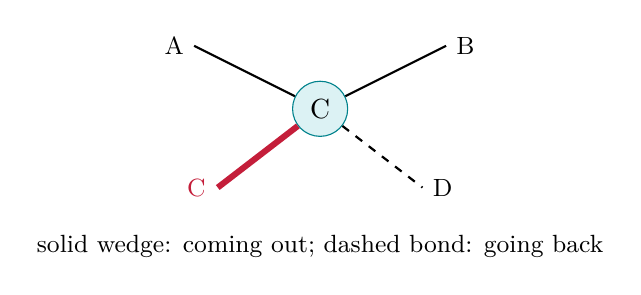
\begin{tikzpicture}[scale=1.0]
  \node[circle, draw=myteal, fill=hdrteal, minimum size=0.7cm] (c) at (0,0) {C};
  \draw[thick] (c) -- (-1.6,0.8) node[left,font=\small] {A};
  \draw[thick] (c) -- (1.6,0.8) node[right,font=\small] {B};
  \draw[line width=2.2pt,myred] (c) -- (-1.3,-1.0) node[left,font=\small] {C};
  \draw[dashed,thick] (c) -- (1.3,-1.0) node[right,font=\small] {D};
  \node[font=\small] at (0,-1.75) {solid wedge: coming out; dashed bond: going back};
\end{tikzpicture}
\end{tcolorbox}

\subsection{Structural Isomers and Stereoisomers}
Structural isomers differ in connectivity, whereas stereoisomers have same connectivity but different spatial arrangement.

\begin{tabularx}{\linewidth}{|B{3cm}|Y|Y|}
\hline
\textbf{Type} & \textbf{Meaning} & \textbf{Example} \\
\hline
Chain isomerism & Different carbon skeleton & n-butane and isobutane \\
\hline
Position isomerism & Functional group at different position & 1-propanol and 2-propanol \\
\hline
Geometrical isomerism & Different arrangement around double bond/ring & cis-2-butene and trans-2-butene \\
\hline
Optical isomerism & Non-superimposable mirror images & lactic acid enantiomers \\
\hline
\end{tabularx}

\subsection{Chirality, Enantiomers and Diastereomers}
A molecule is chiral if it is not superimposable on its mirror image. A common cause is a carbon attached to four different groups.

\begin{tcolorbox}[defbox]
\textbf{Enantiomers} are non-superimposable mirror-image stereoisomers. \textbf{Diastereomers} are stereoisomers that are not mirror images.
\end{tcolorbox}

\subsection{Optical Activity and Absolute Configuration}
Optically active substances rotate plane-polarized light. Absolute configuration is assigned by Cahn-Ingold-Prelog rules.

\begin{tcolorbox}[formulabox, title={Specific Rotation}]
\[
[\alpha]_{\lambda}^{T}=\frac{\alpha}{lc}
\]
where $\alpha$ is observed rotation in degrees, $l$ is path length in dm, and $c$ is concentration in $\mathrm{g\,mL^{-1}}$.
\end{tcolorbox}

\subsection{Elements of Symmetry}
To understand chirality and optical activity, we must analyze the symmetry elements of a molecule. A molecule is chiral (and thus optically active) if and only if it lacks an \textbf{alternating axis of symmetry} ($S_n$). In practice, for most organic molecules, this is equivalent to lacking a \textbf{plane of symmetry} ($\sigma$) and a \textbf{center of symmetry} ($i$).

\begin{tcolorbox}[defbox, title={Symmetry Elements}]
The three primary elements of symmetry are:
\begin{itemize}[leftmargin=*, itemsep=3pt, topsep=2pt]
  \item \textbf{Plane of Symmetry} ($\sigma$): An imaginary plane that bisects a molecule into two halves that are mirror images of each other. Examples include meso-tartaric acid and chlorobenzene.
  \item \textbf{Center of Symmetry} ($i$): A point within a molecule such that any line drawn from any atom through this point meets an identical atom at an equal distance on the opposite side. Examples include trans-1,2-dichloroethylene and trans-1,4-dimethylcyclohexane.
  \item \textbf{Alternating Axis of Symmetry} ($S_n$): An axis such that rotation of the molecule by $360^\circ/n$ followed by reflection across a plane perpendicular to the axis results in a configuration identical to the original.
\end{itemize}
\end{tcolorbox}

\begin{tcolorbox}[tikzbox, title={Symmetry Elements in Common Molecules}]
\centering
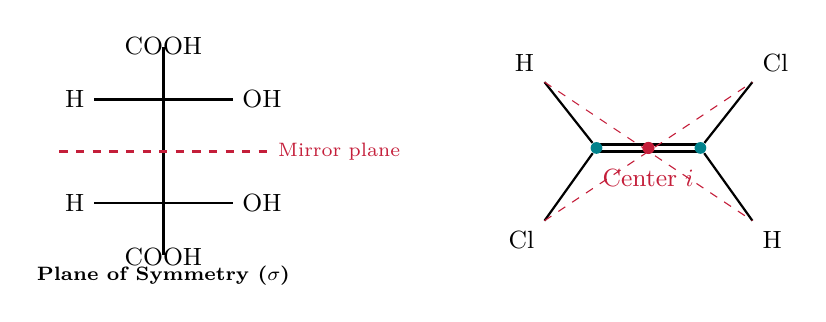
\begin{tikzpicture}[scale=1.1, every node/.style={font=\small}]
  % Plane of symmetry in a simple molecule
  \begin{scope}[shift={(-2.8,0)}]
    \draw[thick] (0,1.2) -- (0,-1.2) node[below, font=\scriptsize\bfseries] {Plane of Symmetry ($\sigma$)};
    \draw[thick] (-0.8,0.6) -- (0.8,0.6);
    \draw[thick] (-0.8,-0.6) -- (0.8,-0.6);
    \draw[thick] (0,1.0) -- (0,-1.0);
    \node[above] at (0,1.0) {COOH};
    \node[below] at (0,-1.0) {COOH};
    \node[left] at (-0.8,0.6) {H}; \node[right] at (0.8,0.6) {OH};
    \node[left] at (-0.8,-0.6) {H}; \node[right] at (0.8,-0.6) {OH};
    \draw[dashed, myred, line width=1.1pt] (-1.2,0) -- (1.2,0) node[right, font=\scriptsize] {Mirror plane};
  \end{scope}

  % Center of symmetry in trans-1,2-dichloroethene
  \begin{scope}[shift={(2.8,0)}]
    \draw[thick] (-0.6,0) -- (0.6,0); % C=C
    \draw[thick] (-0.6,0.08) -- (0.6,0.08);
    \node[circle, fill=myteal, inner sep=1.5pt] (c1) at (-0.6,0.04) {};
    \node[circle, fill=myteal, inner sep=1.5pt] (c2) at (0.6,0.04) {};
    
    \draw[thick] (c1) -- (-1.2,0.8) node[above left] {H};
    \draw[thick] (c1) -- (-1.2,-0.8) node[below left] {Cl};
    \draw[thick] (c2) -- (1.2,0.8) node[above right] {Cl};
    \draw[thick] (c2) -- (1.2,-0.8) node[below right] {H};
    
    \fill[myred] (0,0.04) circle (2pt) node[below=4pt] {Center $i$};
    \draw[dashed, myred, thin] (-1.2,0.8) -- (1.2,-0.8);
    \draw[dashed, myred, thin] (-1.2,-0.8) -- (1.2,0.8);
  \end{scope}
\end{tikzpicture}
\end{tcolorbox}

\begin{tcolorbox}[formulabox, title={Chirality and Symmetry Rule}]
A molecule is chiral and optically active if and only if it is \textbf{dissymmetric} (lacks an alternating axis of symmetry, $S_n$).
\[
\text{Chirality} \iff \text{Absence of } S_n \quad (\text{Practically: absence of } \sigma \text{ and } i)
\]
Note: A molecule can have a simple axis of symmetry ($C_n$) and still be chiral. For example, trans-1,2-dimethylcyclopropane has a $C_2$ axis but no $\sigma$ or $i$, making it chiral and optically active.
\end{tcolorbox}

\subsection{Conformational Analysis}
Conformations arise by rotation about single bonds. Ethane has staggered and eclipsed conformations; staggered is more stable due to lower torsional strain.

\begin{tcolorbox}[tikzbox, title={Ethane Conformations: Staggered and Eclipsed}]
\centering
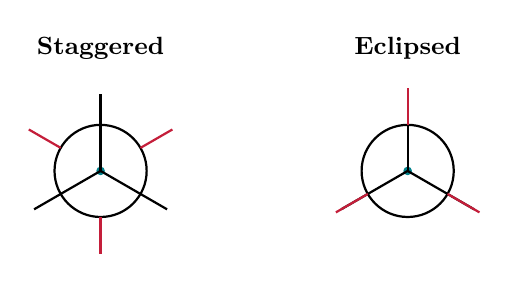
\begin{tikzpicture}[scale=0.78]
  \node[font=\small\bfseries] at (0,2.0) {Staggered};
  \draw[thick] (0,0) circle (0.75);
  \fill[myteal] (0,0) circle (2pt);
  \foreach \a in {90,210,330} \draw[thick] (0,0) -- (\a:1.25);
  \foreach \a in {30,150,270} \draw[thick,myred] (\a:0.75) -- (\a:1.35);
  \node[font=\small\bfseries] at (5,2.0) {Eclipsed};
  \draw[thick] (5,0) circle (0.75);
  \fill[myteal] (5,0) circle (2pt);
  \foreach \a in {90,210,330} {
    \draw[thick] (5,0) -- ($(5,0)+(\a:1.25)$);
    \draw[thick,myred] ($(5,0)+(\a:0.75)$) -- ($(5,0)+(\a:1.35)$);
  }
\end{tikzpicture}
\end{tcolorbox}

\subsection{Isomerism in Transition Metal Compounds}
Coordination compounds show geometrical, optical, linkage, ionization, and coordination isomerism. Square planar and octahedral complexes commonly show cis-trans isomerism.

\begin{tcolorbox}[exambox, title={Exam Points}]
\begin{itemize}[leftmargin=*, itemsep=2pt, topsep=2pt]
  \item Always distinguish structural isomerism from stereoisomerism.
  \item In optical isomerism, mention chirality and non-superimposable mirror images.
  \item CIP assignment needs priority order before clockwise/anticlockwise decision.
  \item For conformational analysis, compare stability using torsional strain.
\end{itemize}
\end{tcolorbox}

% ===============================================================================
\section{Detailed Stereochemical Analysis}
% ===============================================================================

\subsection{Fischer Projection Rules}
Fischer projections are used mainly for molecules with chiral carbon chains. Horizontal bonds come out of the plane toward the viewer; vertical bonds go behind the plane.

\begin{tcolorbox}[tikzbox, title={Fischer Projection Convention}]
\centering
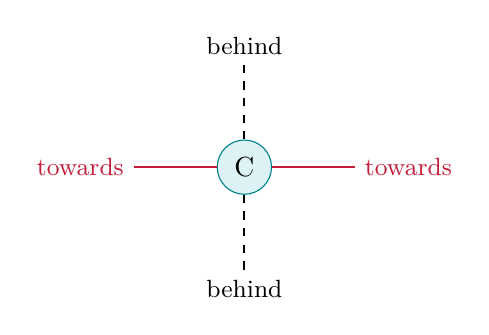
\begin{tikzpicture}[scale=1.0]
  \node[circle, draw=myteal, fill=hdrteal, minimum size=0.6cm] (c) at (0,0) {C};
  \draw[thick,myred] (c) -- (-1.4,0) node[left,font=\small] {towards};
  \draw[thick,myred] (c) -- (1.4,0) node[right,font=\small] {towards};
  \draw[thick,dashed] (c) -- (0,1.3) node[above,font=\small] {behind};
  \draw[thick,dashed] (c) -- (0,-1.3) node[below,font=\small] {behind};
\end{tikzpicture}
\end{tcolorbox}

\begin{tcolorbox}[masonbox, title={Rules for Fischer Projections}]
\begin{itemize}[leftmargin=*, itemsep=2pt, topsep=2pt]
  \item Rotation by $180^\circ$ gives the same molecule.
  \item Rotation by $90^\circ$ gives a different configuration and is not allowed.
  \item Interchanging any two groups once inverts configuration.
  \item Interchanging two pairs of groups gives the original configuration.
\end{itemize}
\end{tcolorbox}

\subsection{Assigning R and S Configuration}
Cahn-Ingold-Prelog priority rules:
\begin{enumerate}[leftmargin=*, itemsep=3pt, topsep=2pt]
  \item Atom directly attached with higher atomic number gets higher priority.
  \item If first atoms are same, compare the next set of attached atoms.
  \item Multiple bonds are treated as equivalent single bonds to duplicate atoms.
  \item View the molecule with the lowest priority group pointing away.
  \item Clockwise order $1\rightarrow2\rightarrow3$ is $R$; anticlockwise is $S$.
\end{enumerate}

\begin{tcolorbox}[examplebox, title={Worked Method: R/S Assignment}]
For a chiral carbon attached to $\mathrm{Br}$, $\mathrm{Cl}$, $\mathrm{CH_3}$, and $\mathrm{H}$:
\[
\mathrm{Br}>\mathrm{Cl}>\mathrm{C}>\mathrm{H}
\]
Place $\mathrm{H}$ away from the viewer. If the order Br $\rightarrow$ Cl $\rightarrow$ $\mathrm{CH_3}$ is clockwise, the configuration is $R$; if anticlockwise, it is $S$.
\end{tcolorbox}

\subsection{Geometrical Isomerism: E/Z and Cis/Trans}
Geometrical isomerism occurs due to restricted rotation around a double bond or within rings. Cis/trans notation is used for simple cases; E/Z notation is used when each double-bond carbon has two different groups.

\begin{tabularx}{\linewidth}{|B{3.2cm}|Y|Y|}
\hline
\textbf{Notation} & \textbf{Meaning} & \textbf{Use case} \\
\hline
Cis & Similar groups on same side & Simple alkenes or rings \\
\hline
Trans & Similar groups on opposite sides & Simple alkenes or rings \\
\hline
E & Higher-priority groups on opposite sides & General alkenes by CIP rule \\
\hline
Z & Higher-priority groups on same side & General alkenes by CIP rule \\
\hline
\end{tabularx}

\subsection{Meso Compounds}
A meso compound contains chiral centres but is optically inactive due to internal symmetry. It is superimposable on its mirror image because optical rotations of two halves cancel internally.

\begin{tcolorbox}[defbox]
\textbf{Meso compound:} An achiral molecule with two or more stereocentres and an internal plane of symmetry.
\end{tcolorbox}

\subsection{Conformational Analysis of Butane}
Butane has anti, gauche, and eclipsed conformations. Anti is most stable because bulky methyl groups are far apart.

\begin{tabularx}{\linewidth}{|B{3cm}|Y|Y|}
\hline
\textbf{Conformation} & \textbf{Dihedral angle between methyl groups} & \textbf{Relative stability} \\
\hline
Anti staggered & $180^\circ$ & Most stable \\
\hline
Gauche staggered & $60^\circ$ & Less stable due to steric repulsion \\
\hline
Eclipsed & $0^\circ$ or $120^\circ$ & Least stable due to torsional strain \\
\hline
\end{tabularx}

\begin{tcolorbox}[examplebox, title={Specific Rotation Numerical}]
If observed rotation $\alpha=+6^\circ$, path length $l=2\ \mathrm{dm}$, and concentration $c=0.5\ \mathrm{g\,mL^{-1}}$:
\[
[\alpha]=\frac{\alpha}{lc}=\frac{6}{2\times0.5}=+6^\circ
\]
\end{tcolorbox}

\subsection{Coordination Compound Stereoisomerism}
Square planar complexes of type $\mathrm{MA_2B_2}$ show cis-trans isomerism. Octahedral complexes may show cis-trans, fac-mer, and optical isomerism depending on ligand arrangement.

\begin{tabularx}{\linewidth}{|B{3cm}|Y|Y|}
\hline
\textbf{Complex type} & \textbf{Possible isomerism} & \textbf{Example pattern} \\
\hline
Square planar $\mathrm{MA_2B_2}$ & Cis-trans & $\mathrm{[Pt(NH_3)_2Cl_2]}$ \\
\hline
Octahedral $\mathrm{MA_4B_2}$ & Cis-trans & Two B ligands adjacent or opposite \\
\hline
Octahedral $\mathrm{MA_3B_3}$ & fac-mer & Three same ligands on one face or meridian \\
\hline
\end{tabularx}

\begin{tcolorbox}[masonbox, title={Stereochemistry Answer Checklist}]
\begin{enumerate}[leftmargin=*, itemsep=3pt, topsep=2pt]
  \item Identify whether connectivity changes or only spatial arrangement changes.
  \item Check for chirality, plane of symmetry, and mirror-image relation.
  \item Use CIP rules for R/S or E/Z configuration.
  \item Mention optical activity only after checking symmetry.
\end{enumerate}
\end{tcolorbox}

\subsection{Number of Stereoisomers}
For a molecule with $n$ independent chiral centres, the maximum number of stereoisomers is:
\[
2^n
\]
If the molecule has internal symmetry, the actual number is less due to meso forms.

\begin{tcolorbox}[examplebox, title={Solved Example: Number of Stereoisomers}]
A molecule has two chiral centres and no plane of symmetry.
\[
\text{Maximum stereoisomers}=2^2=4
\]
These are arranged as two pairs of enantiomers. If a plane of symmetry exists, one or more meso forms reduce the total count.
\end{tcolorbox}

\subsection{Resolution of Racemic Mixtures}
A racemic mixture contains equal amounts of two enantiomers and is optically inactive. Resolution means separation of enantiomers.

\begin{tabularx}{\linewidth}{|B{3.2cm}|Y|Y|}
\hline
\textbf{Method} & \textbf{Principle} & \textbf{Use} \\
\hline
Mechanical separation & Physical separation of crystals & Rare; possible if crystals differ visibly \\
\hline
Chemical resolution & Formation of diastereomeric salts & Common laboratory method \\
\hline
Biochemical resolution & Enzyme reacts with one enantiomer faster & High selectivity \\
\hline
Chromatographic resolution & Chiral stationary phase separates enantiomers & Analytical and preparative use \\
\hline
\end{tabularx}

\subsection{Optical Purity and Enantiomeric Excess}
Optical purity compares observed rotation with rotation of the pure enantiomer.

\begin{tcolorbox}[formulabox, title={Optical Purity}]
\[
\text{Optical purity}=\frac{\alpha_{\mathrm{observed}}}{\alpha_{\mathrm{pure}}}\times100\%
\]
For a two-enantiomer mixture, optical purity is equal to enantiomeric excess.
\end{tcolorbox}

\begin{tcolorbox}[examplebox, title={Solved Example: Enantiomeric Excess}]
If pure enantiomer has specific rotation $+40^\circ$ and mixture shows $+20^\circ$:
\[
\text{optical purity}=\frac{20}{40}\times100=50\%
\]
So enantiomeric excess is $50\%$. The mixture contains $75\%$ major enantiomer and $25\%$ minor enantiomer.
\end{tcolorbox}

\subsection{Sequence Rules for Double Bonds: E/Z Worked Method}
For each double-bond carbon, assign priority to its two substituents using CIP rules. If the two higher-priority groups are on the same side, the alkene is $Z$; if opposite, it is $E$.

\begin{tcolorbox}[examplebox, title={Worked Method: E/Z Assignment}]
For $\mathrm{CH_3CH=CHCl}$, compare substituents on each double-bond carbon. On the left carbon, $\mathrm{CH_3}$ has higher priority than H. On the right carbon, Cl has higher priority than H. If $\mathrm{CH_3}$ and Cl are on opposite sides, the configuration is $E$; if same side, it is $Z$.
\end{tcolorbox}

\subsection{Energy Profile of Butane Rotation}
Rotation about the central C--C bond of butane gives different conformations. Anti is most stable; fully eclipsed is least stable.

\begin{tcolorbox}[tikzbox, title={Qualitative Energy Profile for Butane Rotation}]
\centering
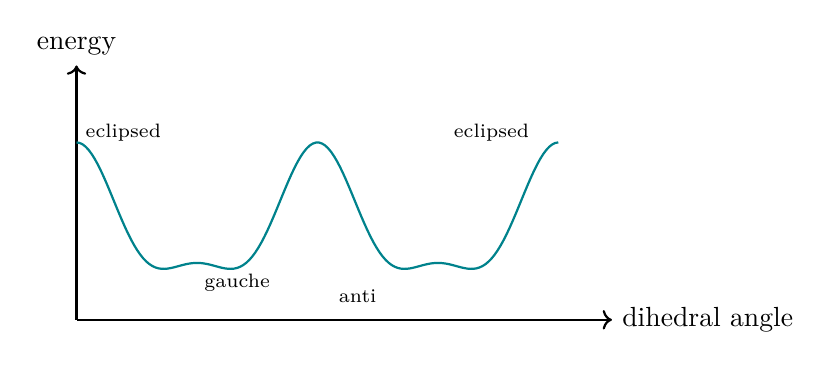
\begin{tikzpicture}[scale=0.85]
  \draw[->, thick] (0,0) -- (8,0) node[right] {dihedral angle};
  \draw[->, thick] (0,0) -- (0,3.8) node[above] {energy};
  \draw[myteal, thick, domain=0:7.2, samples=160]
    plot(\x,{1.4+0.9*cos(100*\x)+0.35*cos(200*\x)});
  \node[font=\scriptsize] at (0.7,2.8) {eclipsed};
  \node[font=\scriptsize] at (2.4,0.55) {gauche};
  \node[font=\scriptsize] at (4.2,0.35) {anti};
  \node[font=\scriptsize] at (6.2,2.8) {eclipsed};
\end{tikzpicture}
\end{tcolorbox}

\subsection{Stereochemistry in Biological and Drug Action}
Many drug molecules are chiral, and different enantiomers can show different biological activity because enzymes and receptors are chiral environments.

\begin{tabularx}{\linewidth}{|B{3cm}|Y|}
\hline
\textbf{Point} & \textbf{Importance} \\
\hline
Different receptor fit & One enantiomer may bind better than the other \\
\hline
Different metabolism & Enzymes may break down enantiomers at different rates \\
\hline
Different toxicity & One enantiomer may be useful while the other causes side effects \\
\hline
Quality control & Optical purity matters in pharmaceutical synthesis \\
\hline
\end{tabularx}

\begin{tcolorbox}[masonbox, title={Previous-Year Style Questions}]
\begin{enumerate}[leftmargin=*, itemsep=4pt, topsep=2pt]
  \item Explain chirality, enantiomers and diastereomers with examples.
  \item State CIP rules and assign R/S configuration for a given molecule.
  \item Explain optical activity, specific rotation and racemic mixture.
  \item Compare conformations of ethane and butane.
  \item Discuss geometrical and optical isomerism in coordination compounds.
\end{enumerate}
\end{tcolorbox}
\newpage
\begin{center}
  {\large\bfseries\color{myred} Quick Revision --- Module 6}\\[3pt]
  {\small\color{mydark} Stereochemistry $|$ BS-CH101}
\end{center}
\noindent{\color{myred}\rule{\linewidth}{1.2pt}}
\vspace{4pt}

\begin{tcolorbox}[formulabox, title={Key Formulas at a Glance}]
\begin{tabularx}{\linewidth}{|B{4.0cm}|Y|}
\hline
\textbf{Formula / Rule} & \textbf{Meaning} \\
\hline
$[\alpha]_{\lambda}^{T}=\displaystyle\frac{\alpha}{lc}$ & Specific rotation of optically active compound. \\
\hline
$\text{enantiomeric excess}=\displaystyle\frac{|R-S|}{R+S}\times100\%$ & Optical purity of a mixture. \\
\hline
$\Delta E=E_{\mathrm{eclipsed}}-E_{\mathrm{staggered}}$ & Torsional energy barrier in conformational analysis. \\
\hline
CIP priority & Higher atomic number gets higher priority. \\
\hline
\end{tabularx}
\end{tcolorbox}

\begin{tcolorbox}[defbox, title={One-Line Definitions}]
\begin{itemize}[leftmargin=*, itemsep=2pt, topsep=2pt]
  \item \textbf{Stereoisomers:} Same connectivity but different spatial arrangement.
  \item \textbf{Chiral molecule:} Molecule not superimposable on its mirror image.
  \item \textbf{Enantiomers:} Non-superimposable mirror-image isomers.
  \item \textbf{Diastereomers:} Stereoisomers that are not mirror images.
  \item \textbf{Optical activity:} Ability to rotate plane-polarized light.
  \item \textbf{Conformation:} Spatial arrangement formed by rotation about single bond.
  \item \textbf{Racemic mixture:} Equimolar mixture of two enantiomers.
\end{itemize}
\end{tcolorbox}

\begin{tcolorbox}[exambox, title={Frequently Asked / Viva Questions}]
\begin{enumerate}[topsep=0pt, label=\textbf{Q\arabic*.}, itemsep=5pt]
  \item \Q{What is stereochemistry?}
    Study of three-dimensional arrangement of atoms in molecules.
  \item \Q{What is chirality?}
    Non-superimposability of a molecule on its mirror image.
  \item \Q{Define enantiomers.}
    Enantiomers are non-superimposable mirror-image stereoisomers.
  \item \Q{Define diastereomers.}
    Diastereomers are stereoisomers that are not mirror images.
  \item \Q{What is optical activity?}
    Rotation of plane-polarized light by a chiral substance.
  \item \Q{What is a racemic mixture?}
    A 1:1 mixture of enantiomers having zero net optical rotation.
  \item \Q{What does R/S configuration indicate?}
    It gives absolute three-dimensional arrangement around a chiral centre.
  \item \Q{Why is staggered ethane more stable than eclipsed ethane?}
    Staggered conformation has minimum torsional repulsion.
  \item \Q{Name isomerism in coordination compounds.}
    Geometrical, optical, linkage, ionization, and coordination isomerism.
  \item \Q{What is geometrical isomerism?}
    Isomerism due to restricted rotation causing cis-trans or fac-mer forms.
  \item \Q{What are the elements of symmetry that determine chirality?}
    A plane of symmetry ($\sigma$), center of symmetry ($i$), and alternating axis of symmetry ($S_n$). A molecule is chiral if and only if it lacks any $S_n$ axis.
  \item \Q{Can a molecule containing chiral carbon atoms be optically inactive?}
    Yes, meso compounds contain chiral carbons but are optically inactive because they have an internal plane of symmetry ($\sigma$), which causes internal compensation of optical rotation.
\end{enumerate}
\end{tcolorbox}

\begin{tcolorbox}[tikzbox, title={Summary Reference Table}]
\begin{tabularx}{\linewidth}{|B{3cm}|Y|Y|}
\hline
\textbf{Pair} & \textbf{Relation} & \textbf{Key difference} \\
\hline
Structural isomers & Different connectivity & Different bonding sequence \\
\hline
Enantiomers & Mirror images & Equal and opposite optical rotation \\
\hline
Diastereomers & Not mirror images & Different physical properties \\
\hline
Conformers & Rotation about single bond & Interconvert without bond breaking \\
\hline
\end{tabularx}
\end{tcolorbox}


% -- Module 7 -----------------------------------------------------------------
\modulestart{7}{Organic Reactions and Drug Molecule Synthesis}

\section{Organic Reactions and Drug Molecule Synthesis}
% ===============================================================================

\begin{tcolorbox}[defbox]
\textbf{Organic reaction mechanism} explains the step-by-step breaking and making of bonds during conversion of reactants into products. It identifies intermediates, reagents, and electron movement.
\end{tcolorbox}

\subsection{Substitution Reactions}
In substitution, one atom or group is replaced by another. Nucleophilic substitution is common in alkyl halides.

\begin{tabularx}{\linewidth}{|B{2.8cm}|Y|Y|}
\hline
\textbf{Type} & \textbf{Main feature} & \textbf{Favoured by} \\
\hline
$\mathrm{S_N1}$ & Two-step, carbocation intermediate & Tertiary substrate, polar protic solvent \\
\hline
$\mathrm{S_N2}$ & One-step backside attack & Methyl/primary substrate, strong nucleophile \\
\hline
\end{tabularx}

\begin{tcolorbox}[tikzbox, title={SN2 Backside Attack Concept}]
\centering
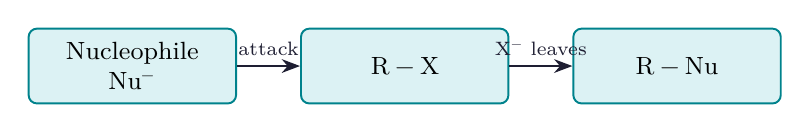
\begin{tikzpicture}[node distance=1.0cm and 0.8cm]
  \node[block] (nu) {Nucleophile\\$\mathrm{Nu^-}$};
  \node[block, right=of nu] (rx) {$\mathrm{R-X}$};
  \node[block, right=of rx] (prod) {$\mathrm{R-Nu}$};
  \draw[arrow] (nu) -- node[above,font=\scriptsize] {attack} (rx);
  \draw[arrow] (rx) -- node[above,font=\scriptsize] {$\mathrm{X^-}$ leaves} (prod);
\end{tikzpicture}
\end{tcolorbox}

\subsection{Addition and Elimination Reactions}
Addition reactions add atoms across multiple bonds. Elimination reactions remove atoms from adjacent carbons to form a double bond.

\begin{tcolorbox}[formulabox, title={Typical Patterns}]
\[
\mathrm{C=C + XY \rightarrow X-C-C-Y}
\]
\[
\mathrm{R-CH_2-CH_2X \rightarrow R-CH=CH_2 + HX}
\]
\end{tcolorbox}

\subsection{Oxidation, Reduction, Cyclization and Ring Opening}
Oxidation increases C-O, C-N, or C-X bonds or decreases C-H bonds. Reduction increases C-H bonds or removes electronegative atoms. Cyclization forms a ring; ring opening converts cyclic compounds into open-chain products.

\begin{tabularx}{\linewidth}{|B{3cm}|Y|Y|}
\hline
\textbf{Reaction} & \textbf{Meaning} & \textbf{Example idea} \\
\hline
Oxidation & Gain of oxygen or loss of hydrogen & Alcohol to aldehyde/acid \\
\hline
Reduction & Gain of hydrogen or loss of oxygen & Carbonyl to alcohol \\
\hline
Cyclization & Ring formation & Intramolecular attack \\
\hline
Ring opening & Cleavage of a ring bond & Epoxide hydrolysis \\
\hline
\end{tabularx}

\subsection{Synthesis of a Common Drug Molecule: Aspirin}
Aspirin (acetylsalicylic acid) is prepared by acetylation of salicylic acid using acetic anhydride in acidic medium.

\begin{tcolorbox}[formulabox, title={Aspirin Synthesis Reaction}]
\[
\mathrm{Salicylic\ acid + Acetic\ anhydride \xrightarrow{H^+} Aspirin + Acetic\ acid}
\]
\end{tcolorbox}

\begin{tcolorbox}[tikzbox, title={Flow Diagram for Aspirin Preparation}]
\centering
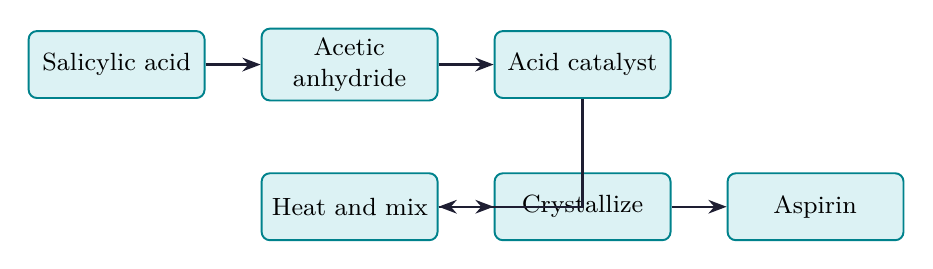
\begin{tikzpicture}[node distance=0.8cm and 0.7cm,
  sblock/.style={rectangle, draw=myteal, fill=hdrteal, text width=2.0cm,
    align=center, minimum height=0.85cm, font=\small,
    rounded corners=3pt, line width=0.7pt}]
  \node[sblock] (s1) {Salicylic acid};
  \node[sblock, right=of s1] (s2) {Acetic anhydride};
  \node[sblock, right=of s2] (s3) {Acid catalyst};
  \node[sblock, below=0.9cm of s2] (s4) {Heat and mix};
  \node[sblock, right=of s4] (s5) {Crystallize};
  \node[sblock, right=of s5] (s6) {Aspirin};
  \draw[arrow] (s1) -- (s2);
  \draw[arrow] (s2) -- (s3);
  \draw[arrow] (s3) |- (s4);
  \draw[arrow] (s4) -- (s5);
  \draw[arrow] (s5) -- (s6);
\end{tikzpicture}
\end{tcolorbox}

\subsection{Synthesis of a Common Drug Molecule: Paracetamol}
Paracetamol (acetaminophen or $p$-acetamidophenol) is a widely used analgesic (pain reliever) and antipyretic (fever reducer). It is synthesized from phenol via a three-step pathway.

\begin{tcolorbox}[defbox, title={Paracetamol Synthesis Reactions}]
The three steps involved in the industrial/laboratory synthesis are:
\begin{enumerate}[leftmargin=*, itemsep=3pt, topsep=2pt]
  \item \textbf{Nitration of Phenol:} Phenol reacts with dilute nitric acid ($\mathrm{HNO_3}$) at low temperature ($\sim 298\ \mathrm{K}$) to yield a mixture of $o$-nitrophenol and $p$-nitrophenol. The para isomer is separated by steam distillation (since the ortho isomer is steam-volatile due to intramolecular hydrogen bonding).
  \item \textbf{Reduction to $p$-Aminophenol:} $p$-nitrophenol is reduced to $p$-aminophenol using reducing agents like iron and hydrochloric acid ($\mathrm{Fe/HCl}$) or tin and hydrochloric acid ($\mathrm{Sn/HCl}$).
  \item \textbf{Acetylation:} $p$-aminophenol is reacted with acetic anhydride ($\mathrm{(CH_3CO)_2O}$) in an aqueous or weakly acidic/basic medium. The amino group ($-\mathrm{NH_2}$) undergoes selective acetylation to yield Paracetamol.
\end{enumerate}
\end{tcolorbox}

\begin{tcolorbox}[tikzbox, title={Reaction Scheme: Phenol to Paracetamol}]
\centering
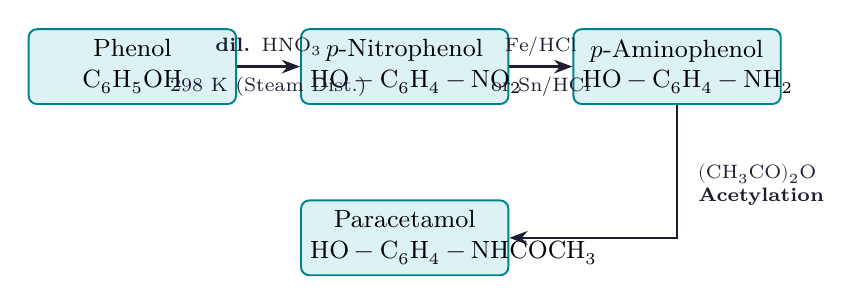
\begin{tikzpicture}[node distance=1.0cm and 0.8cm,
  rxnblock/.style={rectangle, draw=myteal, fill=hdrteal, text width=2.4cm,
    align=center, minimum height=0.95cm, font=\small,
    rounded corners=3pt, line width=0.7pt}]
  \node[rxnblock] (p1) {Phenol\\$\mathrm{C_6H_5OH}$};
  \node[rxnblock, right=of p1] (p2) {$p$-Nitrophenol\\$\mathrm{HO-C_6H_4-NO_2}$};
  \node[rxnblock, right=of p2] (p3) {$p$-Aminophenol\\$\mathrm{HO-C_6H_4-NH_2}$};
  \node[rxnblock, below=1.2cm of p2] (p4) {Paracetamol\\$\mathrm{HO-C_6H_4-NHCOCH_3}$};
  
  \draw[arrow] (p1) -- node[above, font=\scriptsize\bfseries] {dil. $\mathrm{HNO_3}$} node[below, font=\scriptsize] {$298\ \mathrm{K}$ (Steam Dist.)} (p2);
  \draw[arrow] (p2) -- node[above, font=\scriptsize\bfseries] {$\mathrm{Fe / HCl}$} node[below, font=\scriptsize] {or $\mathrm{Sn / HCl}$} (p3);
  \draw[arrow] (p3) |- node[right=4pt, pos=0.3, font=\scriptsize\bfseries, align=left] {$\mathrm{(CH_3CO)_2O}$\\Acetylation} (p4);
\end{tikzpicture}
\end{tcolorbox}

\begin{tcolorbox}[formulabox, title={Selective Acetylation Mechanism (Chemoselectivity)}]
In $p$-aminophenol, both the amino group ($-\mathrm{NH_2}$) and the hydroxyl group ($-\mathrm{OH}$) are nucleophilic. However, nitrogen is less electronegative than oxygen, making the lone pair on nitrogen much more nucleophilic and available for attack. Therefore, acetylation occurs exclusively at the nitrogen atom:
\[
\mathrm{HO-C_6H_4-NH_2 + (CH_3CO)_2O \longrightarrow HO-C_6H_4-NHCOCH_3 + CH_3COOH}
\]
\textbf{Mechanism in Words:}
\begin{enumerate}[leftmargin=*, itemsep=2pt, topsep=1pt]
  \item The nucleophilic nitrogen lone pair of $p$-aminophenol attacks one of the carbonyl carbons of acetic anhydride.
  \item A tetrahedral intermediate is formed.
  \item The carbonyl double bond is restored, and an acetate ion departs as the leaving group.
  \item Deprotonation of the nitrogen atom gives Paracetamol ($p$-acetamidophenol) and acetic acid.
\end{enumerate}
\end{tcolorbox}

\subsection{Mechanistic Exam Language}
For mechanism-based answers, identify electrophile, nucleophile, leaving group, intermediate, and product. Use curved-arrow reasoning in words even when detailed curved arrows are not drawn.

\begin{tcolorbox}[exambox, title={Exam Points}]
\begin{itemize}[leftmargin=*, itemsep=2pt, topsep=2pt]
  \item Compare $\mathrm{S_N1}$ and $\mathrm{S_N2}$ using step, intermediate, rate law, and stereochemistry.
  \item For addition and elimination, write the general reaction pattern.
  \item For oxidation/reduction, state change in C-H and C-O bonds.
  \item For aspirin synthesis, mention salicylic acid, acetic anhydride, acid catalyst, and acetylation.
\end{itemize}
\end{tcolorbox}

% ===============================================================================
\section{Detailed Organic Reaction Notes and Synthesis Planning}
% ===============================================================================

\subsection{Reaction Intermediates}
Organic reactions often proceed through reactive intermediates. Stability of intermediates decides product distribution and rate.

\begin{tabularx}{\linewidth}{|B{3cm}|Y|Y|}
\hline
\textbf{Intermediate} & \textbf{Nature} & \textbf{Stability trend} \\
\hline
Carbocation & Electron-deficient carbon with positive charge & $3^\circ>2^\circ>1^\circ>\mathrm{CH_3^+}$ \\
\hline
Carbanion & Electron-rich carbon with negative charge & Stabilized by electron-withdrawing groups \\
\hline
Free radical & Species with unpaired electron & $3^\circ>2^\circ>1^\circ>\mathrm{CH_3\cdot}$ \\
\hline
Carbene & Neutral divalent carbon species & Highly reactive; addition to alkenes \\
\hline
\end{tabularx}

\subsection{Detailed Comparison of \texorpdfstring{$\mathrm{S_N1}$}{SN1} and \texorpdfstring{$\mathrm{S_N2}$}{SN2}}

\begin{tabularx}{\linewidth}{|B{3.0cm}|Y|Y|}
\hline
\textbf{Point} & \textbf{$\mathrm{S_N1}$} & \textbf{$\mathrm{S_N2}$} \\
\hline
Mechanism & Two-step & One-step concerted \\
\hline
Rate law & $k[\mathrm{RX}]$ & $k[\mathrm{RX}][\mathrm{Nu^-}]$ \\
\hline
Intermediate & Carbocation & No intermediate \\
\hline
Substrate & $3^\circ>2^\circ>1^\circ$ & methyl $>1^\circ>2^\circ$ \\
\hline
Solvent & Polar protic & Polar aprotic \\
\hline
Stereochemistry & Racemization possible & Inversion of configuration \\
\hline
\end{tabularx}

\begin{tcolorbox}[examplebox, title={Solved Concept: Choosing SN1 or SN2}]
Tertiary butyl chloride reacts with water mainly by $\mathrm{S_N1}$ because a stable tertiary carbocation can form and water is a weak nucleophile in polar protic medium. Methyl bromide reacts with $\mathrm{OH^-}$ mainly by $\mathrm{S_N2}$ because backside attack is unhindered.
\end{tcolorbox}

\subsection{Electrophilic Addition to Alkenes}
Alkenes undergo electrophilic addition because the pi bond is electron rich. Addition of HX follows Markovnikov rule in normal ionic addition.

\begin{tcolorbox}[defbox]
\textbf{Markovnikov rule:} In addition of HX to an unsymmetrical alkene, hydrogen attaches to the carbon already having more hydrogen atoms, and X attaches to the more substituted carbon.
\end{tcolorbox}

\begin{tcolorbox}[formulabox, title={Addition of HBr to Propene}]
\[
\mathrm{CH_3-CH=CH_2+HBr\rightarrow CH_3-CHBr-CH_3}
\]
The major product is 2-bromopropane due to formation of the more stable secondary carbocation.
\end{tcolorbox}

\subsection{Elimination: E1 and E2}
Elimination reactions form alkenes. E1 proceeds through carbocation; E2 occurs in one step with base removing beta-hydrogen as leaving group departs.

\begin{tabularx}{\linewidth}{|B{3cm}|Y|Y|}
\hline
\textbf{Point} & \textbf{E1} & \textbf{E2} \\
\hline
Steps & Two-step & One-step \\
\hline
Intermediate & Carbocation & None \\
\hline
Base strength & Weak base possible & Strong base required \\
\hline
Substrate & Tertiary favoured & Primary, secondary, tertiary possible \\
\hline
Stereochemical need & No strict anti requirement & Anti-periplanar H and leaving group preferred \\
\hline
\end{tabularx}

\subsection{Oxidation and Reduction Reagents}
Remembering reagent function is more useful than memorizing long mechanisms for basic engineering chemistry.

\begin{tabularx}{\linewidth}{|B{3cm}|Y|Y|}
\hline
\textbf{Reagent} & \textbf{Type} & \textbf{Common use} \\
\hline
$\mathrm{KMnO_4}$ & Strong oxidizing agent & Alkene oxidation, alcohol oxidation \\
\hline
$\mathrm{K_2Cr_2O_7/H^+}$ & Oxidizing agent & Primary alcohol to acid, secondary alcohol to ketone \\
\hline
$\mathrm{LiAlH_4}$ & Strong reducing agent & Carbonyl and acid derivatives to alcohols \\
\hline
$\mathrm{NaBH_4}$ & Mild reducing agent & Aldehyde/ketone to alcohol \\
\hline
$\mathrm{H_2/Ni}$ & Catalytic reduction & Alkene to alkane \\
\hline
\end{tabularx}

\subsection{Cyclization and Ring Opening}
Cyclization is favoured when the reacting ends of a molecule can form a stable five- or six-membered ring. Ring opening is important for strained rings like epoxides.

\begin{tcolorbox}[tikzbox, title={Cyclization and Ring Opening Concept}]
\centering
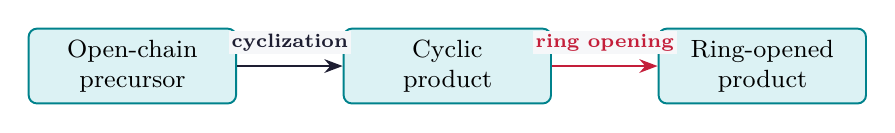
\begin{tikzpicture}[
  rxnlabel/.style={font=\scriptsize\bfseries, fill=mygray, inner sep=1pt}
]
  \node[block] (open) at (0,0) {Open-chain\\precursor};
  \node[block] (ring) at (4,0) {Cyclic\\product};
  \node[block] (open2) at (8,0) {Ring-opened\\product};
  \draw[arrow] (open) -- node[rxnlabel, above=4pt] {cyclization} (ring);
  \draw[redarrow] (ring) -- node[rxnlabel, above=4pt] {ring opening} (open2);
\end{tikzpicture}
\end{tcolorbox}

\subsection{Aspirin Synthesis: Mechanism and Purification}
In aspirin preparation, salicylic acid provides the phenolic $-\mathrm{OH}$ group and acetic anhydride provides the acetyl group. Acid catalyst increases electrophilicity of acetic anhydride. The product is purified by recrystallization.

\begin{enumerate}[leftmargin=*, itemsep=3pt, topsep=2pt]
  \item Protonation of acetic anhydride increases electrophilic character of carbonyl carbon.
  \item Phenolic oxygen of salicylic acid attacks the carbonyl carbon.
  \item Acetate group leaves and deprotonation gives aspirin.
  \item Cold water helps crystallize aspirin because aspirin is less soluble in cold water.
\end{enumerate}

\begin{tcolorbox}[examplebox, title={Aspirin Yield Calculation}]
If theoretical yield is $5.00\ \mathrm{g}$ and actual yield is $3.80\ \mathrm{g}$:
\[
\%\ \text{yield}=\frac{\text{actual yield}}{\text{theoretical yield}}\times100
\]
\[
\%\ \text{yield}=\frac{3.80}{5.00}\times100=76\%
\]
\end{tcolorbox}

\begin{tcolorbox}[masonbox, title={Organic Reaction Answer Checklist}]
\begin{enumerate}[leftmargin=*, itemsep=3pt, topsep=2pt]
  \item Identify substrate, reagent, nucleophile/electrophile, and leaving group.
  \item Classify the reaction as substitution, addition, elimination, oxidation, reduction, cyclization, or ring opening.
  \item Write rate law or regioselectivity rule where applicable.
  \item Mention major product and reason for its formation.
  \item For drug synthesis, include reactants, catalyst, reaction type, purification, and yield idea.
\end{enumerate}
\end{tcolorbox}

\subsection{Reaction Map for Basic Organic Transformations}
Most exam questions ask how one functional group changes into another. The following map gives the common first-year transformations.

\begin{tabularx}{\linewidth}{|B{3.2cm}|Y|Y|}
\hline
\textbf{Conversion} & \textbf{Typical reagent} & \textbf{Reaction class} \\
\hline
Alkene to alkane & $\mathrm{H_2/Ni}$ & Reduction / hydrogenation \\
\hline
Alkene to alcohol & $\mathrm{H_2O/H^+}$ & Addition \\
\hline
Alcohol to alkene & conc. $\mathrm{H_2SO_4}$, heat & Elimination / dehydration \\
\hline
Primary alcohol to acid & $\mathrm{KMnO_4}$ or $\mathrm{K_2Cr_2O_7/H^+}$ & Oxidation \\
\hline
Aldehyde to alcohol & $\mathrm{NaBH_4}$ & Reduction \\
\hline
Alkyl halide to alcohol & aqueous $\mathrm{KOH}$ & Nucleophilic substitution \\
\hline
\end{tabularx}

\subsection{Curly-Arrow Logic in Words}
Even when curved arrows are not drawn, the answer should describe electron flow clearly:
\begin{enumerate}[leftmargin=*, itemsep=3pt, topsep=2pt]
  \item A nucleophile donates an electron pair.
  \item An electrophile accepts an electron pair.
  \item A leaving group departs with the bonding electron pair.
  \item Formation of a stable intermediate or transition state controls the major product.
\end{enumerate}

\begin{tcolorbox}[examplebox, title={Worked Mechanism in Words: Alcohol to Alkene}]
In acid-catalysed dehydration of an alcohol, the $-\mathrm{OH}$ group is first protonated to form a better leaving group, water. Water leaves to form a carbocation. A base removes a beta-hydrogen, and a double bond forms. The major alkene is usually the more substituted alkene according to Zaitsev rule.
\end{tcolorbox}

\subsection{Zaitsev and Hofmann Elimination}
When more than one alkene can form, regioselectivity matters.

\begin{tabularx}{\linewidth}{|B{3cm}|Y|Y|}
\hline
\textbf{Rule} & \textbf{Major product} & \textbf{Typical condition} \\
\hline
Zaitsev rule & More substituted alkene & Small strong base or normal elimination \\
\hline
Hofmann rule & Less substituted alkene & Bulky base or quaternary ammonium elimination \\
\hline
\end{tabularx}

\subsection{Addition to Carbonyl Compounds}
The carbonyl group is polar. Carbon is electrophilic and oxygen is nucleophilic/basic. Nucleophiles attack the carbonyl carbon to form addition products.

\begin{tcolorbox}[tikzbox, title={Carbonyl Addition Concept}]
\centering
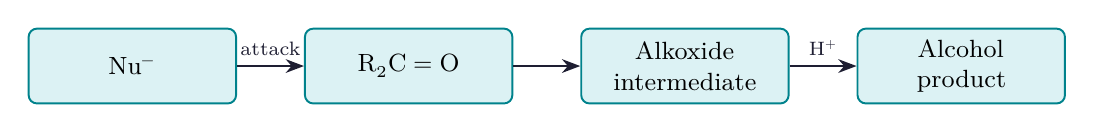
\begin{tikzpicture}[node distance=0.8cm and 0.85cm]
  \node[block] (nu) {$\mathrm{Nu^-}$};
  \node[block, right=of nu] (co) {$\mathrm{R_2C=O}$};
  \node[block, right=of co] (alk) {Alkoxide\\intermediate};
  \node[block, right=of alk] (alc) {Alcohol\\product};
  \draw[arrow] (nu) -- node[above,font=\scriptsize] {attack} (co);
  \draw[arrow] (co) -- (alk);
  \draw[arrow] (alk) -- node[above,font=\scriptsize] {$\mathrm{H^+}$} (alc);
\end{tikzpicture}
\end{tcolorbox}

\subsection{Green Chemistry Note for Drug Synthesis}
Engineering chemistry answers may include practical synthesis quality. A good drug synthesis should be high-yielding, selective, safe, and easy to purify.

\begin{tabularx}{\linewidth}{|B{3cm}|Y|}
\hline
\textbf{Green chemistry point} & \textbf{Meaning in aspirin synthesis} \\
\hline
Atom economy & Prefer maximum incorporation of reactant atoms into product \\
\hline
Safer solvent & Use minimum harmful solvent during purification \\
\hline
Energy efficiency & Avoid unnecessary heating time \\
\hline
Waste reduction & Reduce excess reagent and by-product handling \\
\hline
Product purity & Recrystallization improves purity for medicinal use \\
\hline
\end{tabularx}

\subsection{Tests for Functional Groups}
Short practical-style questions may ask how a functional group is detected.

\begin{tabularx}{\linewidth}{|B{3.2cm}|Y|Y|}
\hline
\textbf{Functional group} & \textbf{Test} & \textbf{Positive observation} \\
\hline
Alkene & Bromine water & Decolorization \\
\hline
Aldehyde & Tollens' reagent & Silver mirror \\
\hline
Carboxylic acid & Sodium bicarbonate & Brisk effervescence of $\mathrm{CO_2}$ \\
\hline
Phenol & Ferric chloride test & Violet or coloured complex \\
\hline
Alcohol & Esterification & Fruity smell of ester \\
\hline
\end{tabularx}

\begin{tcolorbox}[masonbox, title={Previous-Year Style Questions}]
\begin{enumerate}[leftmargin=*, itemsep=4pt, topsep=2pt]
  \item Compare $\mathrm{S_N1}$ and $\mathrm{S_N2}$ mechanisms with stereochemical outcome.
  \item Explain electrophilic addition to propene using Markovnikov rule.
  \item Compare E1 and E2 elimination reactions.
  \item Write short notes on oxidation and reduction reagents in organic chemistry.
  \item Describe aspirin synthesis, purification and percentage yield calculation.
\end{enumerate}
\end{tcolorbox}
\newpage
\begin{center}
  {\large\bfseries\color{myred} Quick Revision --- Module 7}\\[3pt]
  {\small\color{mydark} Organic Reactions and Drug Molecule Synthesis $|$ BS-CH101}
\end{center}
\noindent{\color{myred}\rule{\linewidth}{1.2pt}}
\vspace{4pt}

\begin{tcolorbox}[formulabox, title={Key Formulas at a Glance}]
{\setlength{\tabcolsep}{4pt}\renewcommand{\arraystretch}{1.65}%
\begin{tabularx}{\linewidth}{|B{3.0cm}|Y|}
\hline
\textbf{Formula / Rule} & \textbf{Meaning} \\
\hline
$\text{rate}_{S_N1}=k[\mathrm{RX}]$ & First-order nucleophilic substitution. \\
\hline
$\text{rate}_{S_N2}=k[\mathrm{RX}][\mathrm{Nu^-}]$ & Second-order nucleophilic substitution. \\
\hline
Addition pattern & $\mathrm{C=C+XY\rightarrow X-C-C-Y}$\newline General addition across a multiple bond. \\
\hline
Elimination pattern & $\mathrm{R-CH_2-CH_2X\rightarrow R-CH=CH_2+HX}$\newline Removal of HX to form an alkene. \\
\hline
Aspirin synthesis & $\mathrm{Salicylic\ acid+Acetic\ anhydride\rightarrow Aspirin+Acetic\ acid}$\newline Acetylation reaction for aspirin preparation. \\
\hline
Paracetamol synthesis & $\mathrm{p\text{-}aminophenol + (CH_3CO)_2O \rightarrow Paracetamol + CH_3COOH}$\newline Selective N-acetylation of p-aminophenol. \\
\hline
\end{tabularx}}
\end{tcolorbox}

\begin{tcolorbox}[defbox, title={One-Line Definitions}]
\begin{itemize}[leftmargin=*, itemsep=2pt, topsep=2pt]
  \item \textbf{Nucleophile:} Electron-rich species that attacks electron-poor centre.
  \item \textbf{Electrophile:} Electron-deficient species that accepts electron pair.
  \item \textbf{Leaving group:} Group that departs with electron pair.
  \item \textbf{Substitution:} Replacement of one group by another.
  \item \textbf{Addition:} Addition of atoms across a multiple bond.
  \item \textbf{Elimination:} Removal of groups to form a multiple bond.
  \item \textbf{Acetylation:} Introduction of acetyl group, $\mathrm{CH_3CO-}$.
\end{itemize}
\end{tcolorbox}

\begin{tcolorbox}[exambox, title={Frequently Asked / Viva Questions}]
\begin{enumerate}[topsep=0pt, label=\textbf{Q\arabic*.}, itemsep=5pt]
  \item \Q{What is an organic reaction mechanism?}
    It is the stepwise description of bond breaking and bond formation.
  \item \Q{Define nucleophile.}
    A nucleophile is an electron-rich species that donates an electron pair.
  \item \Q{Define electrophile.}
    An electrophile is an electron-deficient species that accepts an electron pair.
  \item \Q{Compare $\mathrm{S_N1}$ and $\mathrm{S_N2}$ briefly.}
    $\mathrm{S_N1}$ is two-step and forms carbocation; $\mathrm{S_N2}$ is one-step backside attack.
  \item \Q{What is an addition reaction?}
    A reaction in which atoms or groups add across a double or triple bond.
  \item \Q{What is an elimination reaction?}
    A reaction in which small molecules are removed to form a multiple bond.
  \item \Q{How is oxidation recognized in organic chemistry?}
    Increase in C-O/C-X bonds or decrease in C-H bonds.
  \item \Q{How is reduction recognized in organic chemistry?}
    Increase in C-H bonds or decrease in C-O/C-X bonds.
  \item \Q{What is cyclization?}
    Intramolecular reaction leading to ring formation.
  \item \Q{Name reactants used for aspirin synthesis.}
    Salicylic acid and acetic anhydride in presence of acid catalyst.
  \item \Q{Name the starting material and reagents used for Paracetamol synthesis.}
    Phenol is the starting material. Reagents are dilute $\mathrm{HNO_3}$ (nitration), followed by steam distillation to isolate the $p$-nitrophenol isomer, then reduction using $\mathrm{Fe/HCl}$ or $\mathrm{Sn/HCl}$, and finally acetylation using acetic anhydride.
  \item \Q{In Paracetamol synthesis, why does acetylation occur at the $-\mathrm{NH_2}$ group rather than the $-\mathrm{OH}$ group of $p$-aminophenol?}
    Nitrogen is less electronegative than oxygen, making the lone pair on the amino group ($-\mathrm{NH_2}$) more nucleophilic and reactive than the lone pair on the hydroxyl group ($-\mathrm{OH}$). This allows selective N-acetylation under controlled conditions.
\end{enumerate}
\end{tcolorbox}

\begin{tcolorbox}[tikzbox, title={Summary Reference Table}]
{\setlength{\tabcolsep}{4pt}\renewcommand{\arraystretch}{1.55}%
\begin{tabularx}{\linewidth}{|B{4.1cm}|Y|Y|}
\hline
\textbf{Reaction type} & \textbf{Core change} & \textbf{Exam clue} \\
\hline
Substitution & Group replacement & Leaving group present \\
\hline
Addition & Break pi bond, add groups & Alkene/alkyne reactant \\
\hline
Elimination & Remove small molecule & Alkene product \\
\hline
Oxidation/reduction & Change in C-O and C-H bonds & Reagent decides direction \\
\hline
Drug synthesis & Planned sequence & Reactants, catalyst, product \\
\hline
\end{tabularx}}
\end{tcolorbox}


\end{document}
